\documentclass{report}

% Définitions des packages
% Encodage
\usepackage[utf8]{inputenc}
\usepackage[T1]{fontenc}

% Commande spécifique au language français
\usepackage[frenchb]{babel}
\usepackage[autolanguage]{numprint}
\usepackage{hyphenat}


% Autres packages, graphique, etc. 
\usepackage{graphics}
\usepackage{listings}
\usepackage{graphicx}
\usepackage[final]{pdfpages}
\usepackage{xcolor}
\usepackage{layout}
\usepackage[top=3cm, bottom=3cm, left=3cm, right=3cm]{geometry}
\usepackage{float}
\usepackage{titlesec, color}
\usepackage{eurosym}
\usepackage{eso-pic}
\usepackage{listings}
\usepackage{fancyhdr}
\usepackage{hyperref}

\usepackage[toc]{glossaries}


\makeglossaries

% Redéfinitions de macro et commandes
% Nouvelles couleurs
\definecolor{gray75}{gray}{0.75}
\definecolor{RedOrange}{rgb}{255, 99, 71}
\definecolor{Red}{rgb}{192,192,192}
\definecolor{DarkSkyBlue}{HTML}{204A87}



% Nouvelles commandes
\newcommand{\jumpOne}{\\[1\baselineskip]}
\newcommand{\jumpTwo}{\\[2\baselineskip]}

\definecolor{gray75}{gray}{0.75}
\newcommand{\hsp}{\hspace{12pt}}
\titleformat{\chapter}[hang]{\Huge\sffamily}{\thechapter\hsp\textcolor{gray75}{|}\hsp}{0pt}{\Huge}




\renewcommand{\headrulewidth}{1.5pt}

\renewcommand{\footrulewidth}{1pt}




% Photos d'arrière plan sur la couverture. 
\newcommand{\backgroundMain}{
	\put(0,0){
		\parbox[b][\paperheight]
		{\paperwidth}{%
			\vfill
			\centering
			
\includegraphics[
			width=\paperwidth,
			height=\paperheight,
			]{assets/photo_couverture.png}%
			\vfill
		}
	}
}

% Paramètres et styles généraux du rapport. 
% Définitions des paramètres pour le rapport

\pagestyle{fancy}

\hypersetup{
     colorlinks  = true,
     citecolor   = DarkSkyBlue,
     linkcolor   = DarkSkyBlue,
     urlcolor 	 = DarkSkyBlue
}



\pdfminorversion=5 
\pdfcompresslevel=9
\pdfobjcompresslevel=10


% Modifications des titres. 
\titleformat*{\section}{\Large\sffamily\color{black}}
\titleformat*{\subsection}{\large\sffamily\color{gray}}
\titleformat*{\subsubsection}{\itshape\large\sffamily\color{gray}}

\fancyhead[C]{}
\fancyhead[L]{\usefont{OT1}{phv}{m}{n} Master 1 MIAGE 2014/2015}
\fancyhead[R]{\usefont{OT1}{phv}{m}{n} Louis Lainé}

\fancyfoot[C]{\textbf{\thepage}}
\fancyfoot[L]{
\includegraphics[keepaspectratio=true,width=3cm]{assets/logo_bdx.jpg}}
\fancyfoot[R]{
\includegraphics[keepaspectratio=true,width=1.5cm]{assets/miage_bordeaux.jpg}}

% Aucune indentation pour tout le texte
\setlength{\parindent}{0cm}


% Modification de la police
\usefont{OT1}{phv}{m}{n}






\newglossaryentry{elasticsearch}
{name={Elasticsearch}, description={Base de données de type NoSQL orienté document. Elasticsearch est un moteur de recherche libre open source utilisant Lucene.}}

\newglossaryentry{sprint}
{name={sprint},description={Le sprint est une période d'un mois au maximum, au bout de laquelle l'équipe délivre un incrément du produit, potentiellement livrable. Une fois la durée choisie, elle reste constante pendant toute la durée du développement. Un nouveau sprint démarre dès la fin du précédent. Chaque sprint possède un but et on lui associe une liste d'éléments du carnet du produit (fonctionnalités) à réaliser. (Voir partie sur l'agilité).}}

\newglossaryentry{wiki}
{name={wiki},description={Un wiki est une application web qui permet la création, la modification et l'illustration collaboratives de pages à l'intérieur d'un site web. Il utilise un langage de balisage et son contenu est modifiable au moyen d’un navigateur web. C'est un outil de gestion de contenu, dont la structure implicite est minimale, tandis que la structure explicite émerge en fonction des besoins des usagers.}}

\newglossaryentry{newsletter}
{name={newsletter}, description={Une lettre d'information, newsletter ou infolettre est un document d'information envoyé de manière périodique par courrier électronique à une liste de diffusion regroupant l'ensemble des personnes qui y sont inscrites. Une lettre d'information peut également être téléchargée depuis un site web.}}

\newglossaryentry{templates}
{name={template},description={
        Modèle de conception de logiciel ou de présentation des données.
        Synonymes 
        \begin{itemize}
        \item Patron
        \item Modèle
        \item Gabarit
        \end{itemize}}
        }

\newglossaryentry{IDE}
{name={IDE}, description={En programmation informatique, un environnement de développement est un ensemble d'outils pour augmenter la productivité des programmeurs qui développent des logiciels. Il comporte un éditeur de texte destiné à la programmation, des fonctions qui permettent, par pression sur un bouton, de démarrer le compilateur ou l'éditeur de liens ainsi qu'un débogueur en ligne, qui permet d'exécuter ligne par ligne le programme en cours de construction. Certains environnements sont dédiés à un langage de programmation en particulier.}}

\newglossaryentry{vache}{
name={vache à lait},
description={Une vache à lait a part de marché relative élevée sur un marché en faible croissance, en phase de maturité ou en déclin. 
Exigeant peu d'investissements nouveaux et dégageant des flux financiers importants qui devront être réinvesti intelligemment sur les vedettes et les dilemmes}
}


\newglossaryentry{part de marche en valeur}
{name={part de marché en valeur}, description={La PDM valeur ou part de marché valeur désigne la part de marché d’un produit exprimée en valeur monétaire et non en quantité.}}


\newglossaryentry{depot}
{name={dépôt git}, description={Les dépôts distants sont des versions de votre projet qui sont hébergées sur Internet ou le réseau. Vous pouvez en avoir plusieurs, pour lesquels vous pouvez avoir des droits soit en lecture seule, soit en lecture/écriture. Collaborer avec d'autres personnes consiste à gérer ces dépôts distants, en poussant ou tirant des données depuis et vers ces dépôts quand vous souhaitez partager votre travail.}}


\newglossaryentry{commit}
{name={commit},description={Le terme anglais commit désigne une validation de transaction qui fait référence à la commande synonyme Commit présente dans la plupart des systèmes de gestion de base de données et des logiciels de gestion de versions. Dans les systèmes de bases de données et de révision de fichier, la validation est une exécution de la tâche préalablement confiée, marquant à la fois la fin de la demande de transaction et le début de l’exécution de la tâche confiée, qui devra être exécutée atomiquement.}}



\begin{document}
    
    
\begin{titlepage}

\AddToShipoutPicture*{\backgroundMain}


\begin{center}

    % Bottom of the page
    \usefont{OT1}{phv}{m}{n}
    
    \begin{minipage}{.5\textwidth}
    	\begin{flushleft}
    		
\includegraphics[width=0.5\textwidth]{assets/logo_bdx.jpg}~\\[1cm]
    	\end{flushleft}
    \end{minipage}% 
    \begin{minipage}{.5\textwidth}
    	\begin{flushright}
    		
\includegraphics[width=0.6\textwidth]{assets/miage_bordeaux.jpg}~\\[1cm]
    	\end{flushright}
    \end{minipage}
    
    \\[12\baselineskip] 

    % Title
    \HRule \\[0.4cm]
    { \huge \bfseries Pilotage de la qualité dans le développement de projet informatique\\[0.4cm] }

    \HRule \\[2cm]
    
\includegraphics[scale=0.5]{assets/bob_logos.png}
    \\[2cm]

    % Author and supervisor
    \begin{minipage}{0.4\textwidth}
      \begin{flushleft} \large
        Louis Lainé\\
        M1 Miage Bordeaux \\
        Promo 2015 
      \end{flushleft}
    \end{minipage}
    \begin{minipage}{0.4\textwidth}
      \begin{flushright} \large
        Maxime Sénécat \\
        Malo Pichot \\
        Fred Wolf \\
      \end{flushright}
    \end{minipage}

    \vfill


    % Bottom of the page
    {\large 4 Mai 2015 — 29 Août 2015} \\
    {\large Université de Bordeaux. }

\end{center}



\end{titlepage}

    
    \usefont{OT1}{phv}{m}{n}


\chapter{Remerciements}

En premier lieu, je souhaite adresser mes plus sincères remerciements à l'ensemble de l'équipe de Bob el Web.
\jumpOne
Je tiens à remercier chaleureusement, \textbf{Jean-luc Mirebeau} qui m'a accordé sa confiance et permis d'intégrer l'équipe pour ce stage.
\jumpOne
Je souhaite également remercier \textbf{Maxime Sénécat} mon maitre de stage, \textbf{Fred Wold} et \textbf{Malo Pichot} pour leurs conseils, qui m'ont beaucoup aidé durant ce stage. 
\jumpOne
Je souhaite également remercier \textbf{Guillaume Bobinnec}, \textbf{Maëva Bonnier}, \textbf{Johanna Picaud} et \textbf{Laura Früh} pour leur bonne humeur et professionnalisme. 

Un merci à Mr \textbf{Jean Jacques Gillon} pour sont suivi pendant le stage et ses conseils ainsi que l'équipe pédagogique de la MIAGE Bordeaux, qui m'a permis par le biais de ce stage, d'enrichir mon expérience professionnelle.   




    
    \tableofcontents
    
    
\chapter{Summary}

\section{Français}

Au cours du stage que j’ai réalisé au sein de la société Bob El Web, j’ai été chargé de travailler au développement de nouvelles fonctionnalités sur le logiciel Purple Base à partir du logiciel déjà existant, Bob Booking.

Pour apporter des éléments de réponse aux questions de l'équipe technique, en particulier pour
proposer la mise en place de nouvelles solutions de stockage et de traitement de données mettre en place un outillage de test développer un outil de création d'emailing répondre à un cahier des charges.  
J’ai du accumuler un certain nombre de connaissances et rechercher les "bonne pratiques" à mettre en place.
 
Confronté aux difficultés de conception d'un logiciel, je me suis concentré sur les bonnes pratiques à respecter, du début d’un projet et tout au long de son développement. 
Cette expérience de développement d'un nouvel applicatif à partir d’un l'applicatif existant, m'a amené à porter ma réflexion sur plusieurs sujets :

\begin{itemize}
\item Quelle architecture utiliser pour un nouveau projet ? 
\item Comment penser sa maintenance à long terme ? 
\item Comment anticiper les possibilités d'évolutions? 
\end{itemize}

Pour surmonter ces difficultés, les nombreux échanges et la concertation avec l'équipe technique de Bob Booking ont été précieux. 
Ils m’ont permis de prendre en compte leurs expériences antérieures de développeurs et de réfléchir sur des concepts, démarches et outils permettant de concevoir un projet informatique sur de meilleures bases. 

Dans mon rapport de stage je vais chercher à montrer comment la réflexion centrée sur ces concepts m'a aidé à trouver de meilleures pratiques d'un point de vue technique et fonctionnel sur le développement d'un projet informatique, dans le but d'obtenir un logiciel de qualité maintenable et évolutif

Dans le chapitre 3, je présenterais l'entreprise et son activité. 

Le chapitre 5, sera consacré au pilotage de la qualité d'un point de vue "technique" en abordant les problèmes liés à une négligence de la qualité, le concept de dette technique et les solutions à suivre pour minimiser la dette technique sur les projets.

Le chapitre 6, sera consacré à montrer comment l'utilisation de la méthode Agile dans la gestion de projet m'a permit d'apprendre à mettre en oeuvre l'ensemble des pratiques abordés dans le chapitre 5.
Comment à l'aide de cette gestion de projet, il est facile d'intégrer ces méthodes durant le cycle de développement du logiciel et donc d'avoir un pilotage de la qualité vraiment efficace.


\section{Anglais}

During my internship in Bob el Web, I had to work on the new product called "Purple Base", on which I had to develop new features. 

To provide anwsers for the technical team, especially about storage solutions, data processing or set up a test workflow for the Purple Base application, develop an emailing tool. 

I had to accumulate a certain amout of knowledge and look for "good practices" to implement. 

Faced with software design challenges, I focused on good practices to work with from the beginning of the project and throughouts its development. 

This development experience brought me to think about several topics : 

\begin{itemize}
\item What architecture to use for a new project ? 
\item How to think about the long-term maintenance for the project ?
\item How to anticipate the possibilities of changes ?
\end{itemize}

To overcome theses difficulties, the exchanges and cooperation with the technical team was very helpful. 

They shared with me their developer experience which allowed me to reflect on concepts, approaches and tools for designing IT project on a better footing. 


In this report, I will try to show you how the reflection centered on these concepts, helped me to find best practices from a technical and a functional point of view on the development of IT projects, in order to obtain a maintanable and scalable software. 

Chapter 3, will introduce the company and the business. 

Chapter 5, will be devoted to quality on a technical point of view, talking about issues caused by a lack of quality in software development, the concept of technical debt and the solutions to follow in order to minimize technical debt on projects. 

Chapter 6, will be dedicated to show, how the use of Agile in project management allowed me to learn how to implement all the practacices discussed in chapter 5. 
By using this type of project management, it is easy to integrate these methods in the software development cycle and have an effective quality control. 
    
    \usefont{OT1}{phv}{m}{n}

% Parler des produits d'abord. 
% Parler de Bob Booking d'abord, puis les autres produits. 

\chapter{Introduction}

\section{La société}

\subsection{Historique}
Basée à Bordeaux, la société \textbf{Bob el web} est une SAS de 10 salariés créée en 2006 par Jean-Luc Mirebeau et Fred Wolf.
L'activité principale de la société consiste à développer et commercialiser des logiciel de gestion de type CRM (customer relationship management). 

L'expérience de M. Mirebeau dans le monde du spectacle, étant lui-même anciennement "tourneur", lui a permis d’établir le constat que l'organisation d'événements pourrait être plus rapide si les outils informatiques utilisés étaient réunis au sein d'une même plateforme. Il s'est donc lancé dans la création du logiciel Bob Booking.


\subsection{Activité}

L'activité de l'entreprise est centrée autour de la vente de logiciel CRM en B2B (business to business) à destination des professionnels du spectacle en particulier les "tourneur".


\subsubsection{Qu'est-ce qu'un tourneur ?}
Le tourneur imagine, propose et gère une série de spectacles d'un artiste sur un territoire, auprès de lieux de diffusion et sur une période donnée. Il coordonne les efforts de différents programmateurs et promoteurs locaux. Il peut être producteur du spectacle et directement travailler avec les artistes ou bien représenter d'autres producteurs auprès des diffuseurs. Il administre une tournée, y compris les aspects logistiques, techniques et financiers. Il communique auprès de partenaires variés pour valoriser les projets qu'il présente et commercialise des représentations.

\subsubsection{Produits}
Il existe actuellement plusieurs produits proposés et commercialisés par l'entreprise sous forme d'application web (accessible depuis internet et par le biais d'un abonnement).

Chaque produit a des fonctionnalités différentes et vise une cible différente correspondant à un métier spécifique du monde du spectacle.

\newpage


\subsubsection{Bob Booking}

\begin{figure}[h!]
	\centering
	
\includegraphics[width=0.2\textwidth]{assets/booking.png}
\end{figure}


Bob Booking représente le produit ayant des parts de marché élevées sur un marché en faible croissance. 
Ce produit exige peu d'investissements de la part de la société et dégage des flux financiers importants.
C'est la véritable \textbf{\gls{vache} de l'entreprise} 
\jumpTwo
Bob Booking est un outil de communication et de relation commerciale où tout est conçu pour agir efficacement sur l’ensemble des fichier de contacts client.
C’est aussi un outil performant de booking.
Permettant de gérer les tournées et prévisions budgétaires qui s’affichent en temps réel, exportables sous tout types de formats.

C’est enfin un outil d’administration et de régie avec un cycle automatisé de confirmation / contrat / facture, la gestion des équipes sur la route et des VHR.



\begin{figure}[h!]
    \centering
    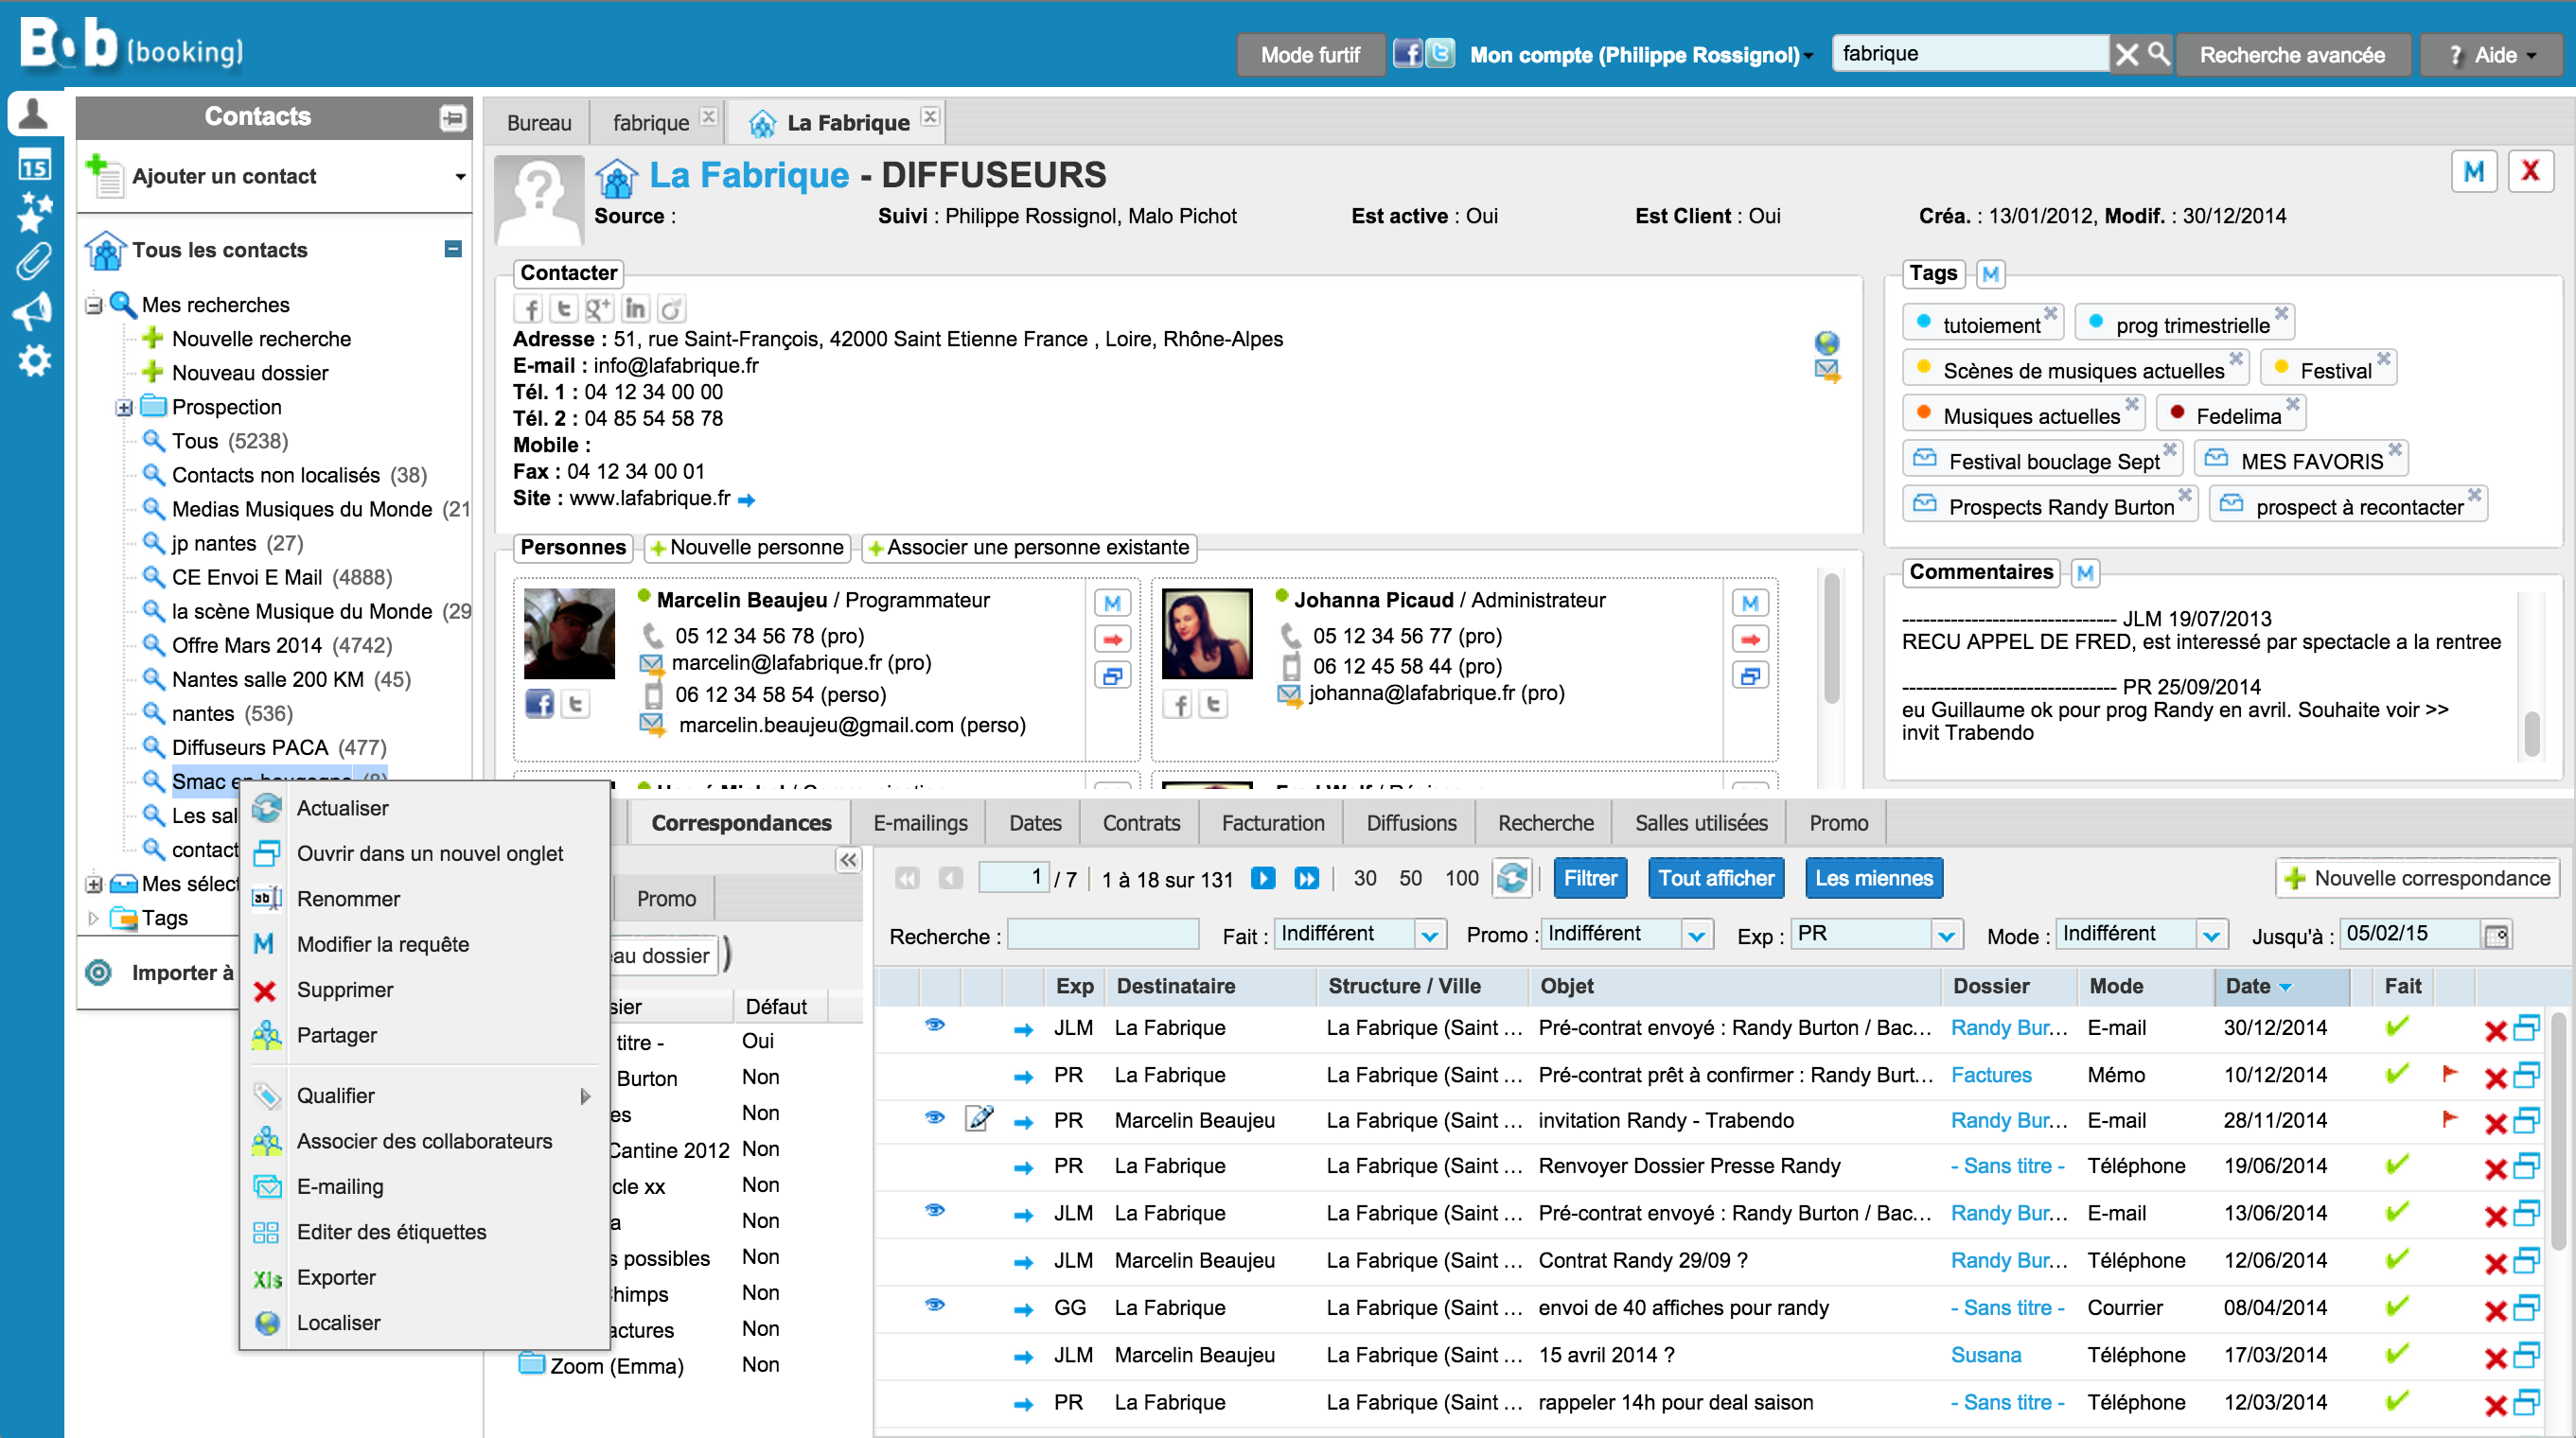
\includegraphics[width=1\textwidth]{assets/bob_screenshot.png}
    \caption{Capture d'écran du logiciel Bob}
    \label{fig:my_label}
\end{figure}

Le logiciel propose ainsi de multiples fonctionnalités

\begin{itemize}
    \item Import et gestion de contact
    \item Recherches avancées à travers l'ensemble des contacts. 
    \item Dossiers de relance et historiques
    \item Envoi d'email
    \item Gestion des campagnes d'emailing ciblés et tracés.
    \item Gestion electronique des documents
    \item Agenda Collaboratif
    \item Comptes, gestions des permissions
    \item etc.
\end{itemize}

Les produits suivants, sont des versions différentes du produit Bob Booking, adapté en fonction des besoins. 


\begin{minipage}{0.3\textwidth}
	\begin{figure}[H]
		\centering
		
\includegraphics[width=0.8\textwidth]{assets/express.png}
    \end{figure}
\end{minipage}%
\begin{minipage}{0.6\textwidth}

% Parti du constat que des les petites structures ne veulent pas toutes les fonctionnalités 
% proposés par Bob. C'est une version minimale 

C'est une version minimale de Bob Booking comprennant uniquement les fonctionnalités principales. 

Bob Express est réservé aux structures émergentes (indépendants, auto-entrepreneurs...) et aux entreprises de l’économie sociale et solidaire.
\end{minipage}

\vspace{5mm}


\begin{minipage}{0.3\textwidth}
	\begin{figure}[H]
		\centering
		
\includegraphics[width=0.8\textwidth]{assets/festival.png}
    \end{figure}
\end{minipage}%
\begin{minipage}{0.6\textwidth}
Bob Lieu \& Festival a été conçu pour centraliser, enrichir et partager toutes les informations et actions nécessaires à la gestion d’événements culturels.

Scénarios de programmation, communication massive vers les fichiers publics, gestion multi-lieux et multi-projets, tâches techniques, affectation des bénévoles ou des intermittents, horaires et ressources techniques…
\end{minipage}

\begin{figure}[h!]
    \centering
    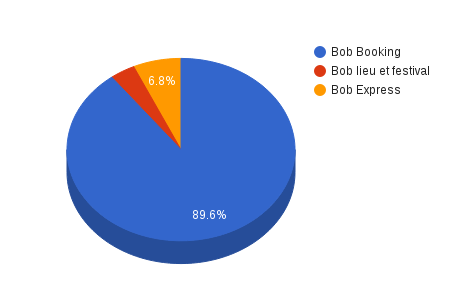
\includegraphics[width=0.8\textwidth]{assets/repartition_client.png}
    \caption{Répartition des clients sur les produits}
    \label{fig:my_label}
\end{figure}

\newpage


\subsection{Purple Base}

Depuis quelques mois l'entreprise travaille à la création d'un nouveau logiciel (dont la sortie est prévu à la fin de l'année 2015), appelée Purple Base. 

\subsubsection{Contexte}
 L'entreprise se retrouve face à la situation ou Bob Booking, a saturé le marché du booking avec environ 50\% de \gls{part de marche en valeur}.
Il est urgent pour l'entreprise de trouver un nouveau relai de croissance. 

En ciblant une nouvelle clientèle : les indépendants, les groupes auto-diffusés.
En proposant avec des technologie de pointes, la mise à disposition d'informations commerciale sur le secteur du booking.

Purple Base est un référentiel de données commerciale du secteur musical,  mis à jour en permanence. 
En présentant une interface nouvelle centralisant les informations des petites structures, l'entreprise souhaite révolutionner le booking indépendant et prendre un nouveau départ. 


% Présentation de purple base, pourquoi ? 
% Réponses de JLM
% Evol du CA -> DONE 
% Présentation de Purple Base 
%Pourquoi ? 
%2 objectifs. 
%- Technologique ; contribuer à un renouveau de l'entreprise en réecrivant la technologie associé (les technologie utilisés se basent sur des techno assez vieilles). 
%- Cible différente (Bto2), petit produit pour groupe auto-diffusé
%--> Offre révolutionner le booking indé. 
%- L'entreprise à une cible + large et veut tailler des part de marchés à des concurrents. 
%C'est quoi ? 
%Référentiel de données, mit à jour en permanence avec les meilleurs données du secteur, une interface toute nouvelle, permettant d'avoir tout au même endroit.
%Comment PB est venu à l'idée ? 
%- Bob booking a saturé le marché du booking avec + de 40/50 \% de PDM en valeur. 
%ainsi il était nécessaire d'avoir un relai de croissance. 
%- Ainsi PB a été l'occasion de choper d'autres part de marché et tout refaire technologiquement

\subsubsection{Architecture}

D'un point de vue architecture, Purple Base se base sur l'application Bob Booking (par le biais d'une Api) pour réaliser les actions sur le serveur. 

Purple Base ayant des fonctionnalités commune avec les logiciels déjà développés, le but étant de se baser sur Bob Booking pour ne pas tout refaire depuis le début et donc gagner du temps. 

\begin{figure}[h!]
\centering
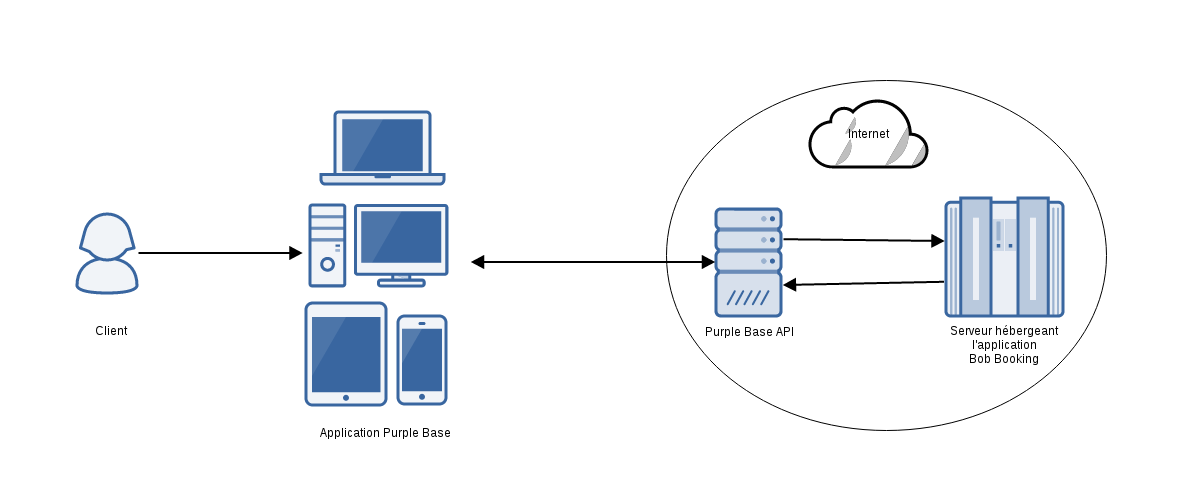
\includegraphics[width=1\textwidth]{assets/archi_pb.png}
\caption{Représentation de l'architecture du logiciel}
\label{fig:my_label}
\end{figure}


\subsubsection{Chiffre d'affaire}

\begin{figure}[h!]
\centering
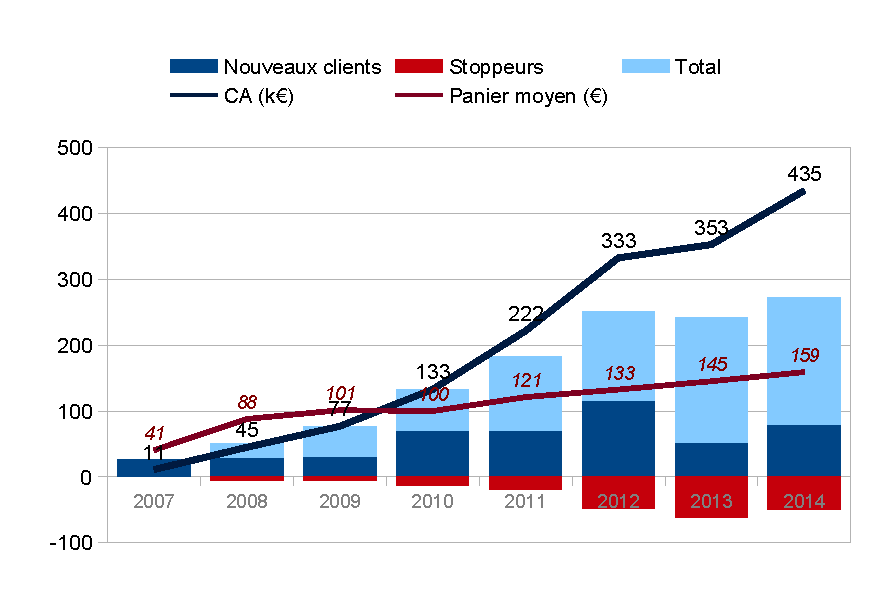
\includegraphics[width=0.8\textwidth]{assets/evol_ca_bob.pdf}
\caption{Evolution du CA depuis la création de l'entreprise}
\label{fig:my_label}
\end{figure}

\subsubsection{Répartition du chiffre d'affaire en 2014}

\begin{minipage}{.6\textwidth}
    \begin{description}
        \item[Prestation de coproduction]
        {5\% du CA est représenté par ces coproduction. 
        Ce sont des prestations que l'entreprise réalise à la demande des clients. Une nouvelle         fonctionnalité qu'un client voudrait avoir dans sont application.
        }
        \item[Vente crédit d'emailing]
        {9\% du CA est représenté par la vente de crédit d'emailing. 
        L'application Bob Booking permet de gérer des campagnes d'emailing. 
        Chaque email envoyé depuis l'application nécessite du crédit. 1 crédit = 1 destinaire d'une campagne. 
        Par exemple pour envoyer 10 campagne à 2000 destinataires, nécessitera 20 000 crédits. 
        }
        \item[Formation client]
        {18\% du CA est représenté par des formations sur les différents logiciels proposés. 
        }
        \item[Nouveaux abonnements]
        {
        Durant l'année 2014, 11\% du CA est représenté par de nouveaux abonnements. Des nouveaux         clients qui ont souscrit pour un Bob Booking ou Express, etc. 
        }
        \item[Abonnements]
        {
        57\% du chiffre d'affaire est représenté par les abonnements des anciens clients. 
        }
        
    \end{description}
\end{minipage}% This must go next to `\end{minipage}`
\begin{minipage}{1\textwidth}
    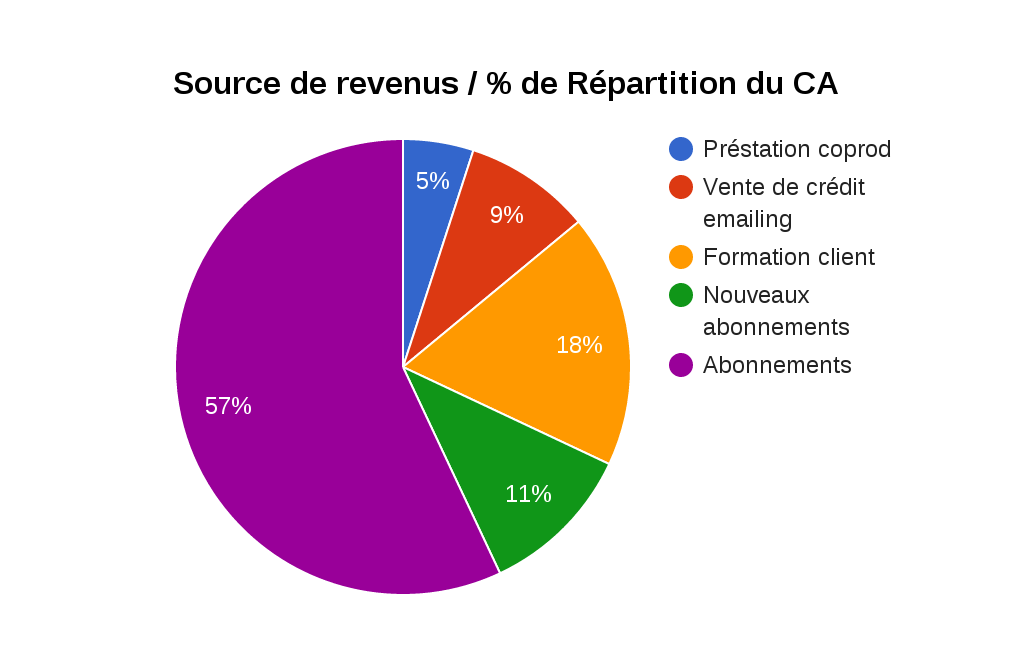
\includegraphics[width=0.65\textwidth]{assets/repartition_ca.png}
\end{minipage}




    
    \usefont{OT1}{phv}{m}{n}

\chapter{Missions}

\section{Commande initiale}

C'est dans le contexte de la nouvelle application Purple Base que j'ai été recruté en stage. 
Ce logiciel devant être une application multi-plateforme j'étais en charge de développer la version tablette. 

Mais les fonctionnalités devant être adaptées sur tablette n'étant pas prête le jour de mon arrivé, j'ai donc travaillé sur d'autres missions tout au long de mon stage. 


\section{Missions réalisées durant le stage}

\subsection{Mise en place du référentiel}

% Pourquoi ?
Ma première mission fut de réfléchir à la mise en place d'une solution de stockage et de traitement de données dans le cadre du référentiel de données pour Purple Base. 
Une base de données avait déjà été selectionnée par l'équipe de développeurs appelée \gls{elasticsearch} 
pour ses capacités à pouvoir traiter et stocker de très grosses masses de données. 

% Qu'est-ce qui a été fait ? 
Pendant un \gls{sprint} je me suis plongé dans diverses ressources, avec comme but de collecter un maximum de connaissances sur \gls{elasticsearch}. 

Ce fut l'occasion de lire un livre sur le fonctionnement détaillé de la base de données, mais également de parcourir blogs et site diverses sur le sujet.

Puisque le fruit de mes recherches est destiné aux autres développeurs, il était primordial qu'une restitution écrite soit fournie, en plus de celle orale à la fin du sprint.
J'ai par conséquent documenté tout ce le travail effectué, sur le \gls{wiki} pour permettre à l'équipe d'avoir une trace du travail réalisé.

% Solutions trouvés
Cette phase de recherche ma permis de pouvoir accumuler des connaissances pour pouvoir répondre aux questions de l'équipe technique. 
J'ai également du me concentrer sur l'aspect "bonne pratiques" à mettre en place pour proposer une base solide et évolutive de la base données.  


\subsection{Outillage de test}
La seconde mission qui m'a été confiée fût de réfléchir à la mise en place de l'outillage de test sur Purple Base. 

% Pourquoi ? 
Pour que Purple Base soit vraiment le renouveau de Bob el Web, le pilotage de la qualité ne doit pas être mis à part. 
En effet, en ne négligeant pas cet aspect, le logiciel aura des bases solides et pourra être maintenable sur le long terme. 
\jumpOne
% Qu'est-ce qui a été fait ? 
Plusieurs sprints ont été consacrés à la recherche d'une solution pour mettre en place un processus de test fiable et évolutif dans le temps. 
Après avoir étudié plusieurs framework de test, j'ai sélectionné à l'aide de mon maitre de stage, Karma et Jasmine (deux framework spécialisé dans le test JavaScript, AngularJS), pour leur flexibilité et facilité d'utilisation. 

% Solutions trouvés et concepts abordés
Cette seconde mission a encore une fois été l'occasion d'alterner phases de recherche et phase de rédaction sur le wiki. 
Ce fut l'occasion pour moi, de me concentrer sur les bonnes pratiques du test à mettre en place sur des applications utilisant la technologie JavaScript/AngularJS. 
% Annexes screenshot wiki et bonnes pratiques. 


\subsection{Newsletter}

% Pourquoi ?

Dans le cadre de l'application Purple Base et de ses nouvelles fonctionnalités, j'ai dû travailler sur le développement d'un outil de création d'emailing. 

En août 2014, la société à réalisé un sondage sur les clients, pour connaitre quelles étaient les fonctionnalités les plus demandés dans Bob Booking. 
La possibilité de pouvoir créer et deployer par le biais d'un outil, des campagnes de communication numérique est apparu dans les premières position.
 

\subsubsection{Qu'est-ce qu'un outil d'emailing ?}
Ce logiciel, permet de créer des \gls{newsletter}, à l'aide de \gls{templates}.
Il permet d'automatiser l'envoi de mails, d'intégrer les contenus sur les réseaux sociaux mais aussi de gérer des fichiers de contacts et de faire du suivis statistique des campagnes envoyées. 

\subsubsection{Pourquoi l'e-mailing?}
C'est un moyen très simple et peu cher de faire connaitre un produit ou un projet sur internet.
Cette méthode consiste à envoyer des emails à des personnes, leur proposant le dit produit ou le projet. 
Les emails, vont permettre de très facilement cibler la population souhaitée qui serait le plus à même d'être touchée par notre produit. 

\paragraph{Exemple} Je vends un concert de Rock d'un groupe des années 80, j'aimerai donc envoyer des emails à mes clients, dans une tranche d'âge spécifique appreciant ce style musical. 

Il est évident que l'on ne va pas rédiger chaque email à la main. 
De même pour la création de l'email qui demande beaucoup de temps des compétences en design pour pouvoir réaliser quelque chose d'esthetique et professionnel. 

C'est là où l'outil de création rentre en jeu !

A partir de template pré-construit, on va pouvoir créer notre mail, ajoutant des images du texte, des liens, etc. 
% Annnexe : newsletter BOB
Cet email va pouvoir par la suite être envoyé à autant de personne souhaité (10 000, 20 000, etc) très facilement par le biais d'un système interne. 

% Qu'est-ce qui a été fait ? 
\subsubsection{Le projet}
L'entreprise avait prévu d'internaliser le développement de la partie gestion des envois, mais le créateur d'email lui, de par sa complexité a initialement été externalisé.

On m'a donc confié la réalisation du chiffrage, la rédaction du cahier des charges (écrit avec le patron de l'entreprise) % annexe : Mettre en annexe, cahier des charges et chiffrage. 
et rechercher un prestataire pour réaliser l'outil. 

Plusieurs prestataires ont répondu à l'appel, cependant soit leur prix ou leur disponibilité ne convenaient pas à l'entreprise. 
Etant à quelques semaines de la fin du stage, j'ai proposé l'idée que je pouvais moi même développer l'outil.
Cette idée a par la suite été acceptée.
J'allais pouvoir m'appliquer à ne pas négliger le coté pilotage de la qualité, étant donné que je passais du rôle de client à prestataire. 

% Concepts abordés
Cette dernière mission m'a vraiment permis de me concentrer sur des questions de bonnes pratiques de la qualité à mettre en place dès le début du développement et celles qu'il est nécessaire de suivre par la suite tout au long du projet. 
C'est aussi celle qui m'a permis de dégager la problématique liée à mon stage. 

\section{Problématique liés aux missions}
C'est donc tout naturellement que j'ai décidé d'orienter ma problèmatique vers le pilotage de la qualité. 
\jumpOne
Ces expériences de développement d'un nouvel applicatif à partir de l'existant (Bob Booking développé par la société en 2007), m'a confronté aux difficultés de conception d'un logiciel.
J'ai du porter ma réflexion sur plusieurs sujets tels que : 
\begin{itemize}
\item Quelle architecture utiliser pour un nouveau projet ? 
\item Comment penser sa maintenance à long terme ? 
\item Comment anticiper les possibilités d'évolutions 
\end{itemize}
Pour surmonter ces difficultés, la communication avec l'équipe technique ma permis de réfléchir en prenant en compte leurs expériences antérieurs de développeurs avec ses échec et ses réussites. 




    
    \chapter{Pilotage de la qualité}

% 
% Changer cette partie, pour la mettre dans une partie dédiée. 

\section{Dette technique}
La dette technique, est un concept reprenant le principe de la dette appliqué au domaine du développement logiciel.

\subsection{Présentation}

Un projet de développement d'une application inclut une conception logicielle (qu'elle soit formalisée ou pas).

Cette dernière fait partie de la qualité du projet. Écrire le code source en suivant la conception définie en amont lui permet d'être cohérent et de faciliter la maintenance :

\begin{itemize}
\item maintenance corrective : corriger les bug informatiques
\item maintenance évolutive : ajouter de nouvelles fonctionnalités au logiciel. 
\end{itemize}

Ainsi, un non-respect de la conception, intentionnel ou non, induit des coûts supplémentaires dans le futur. 
Ce sont les intérêts. C'est pourquoi l'on parle de dette technique, pour montrer l'analogie avec la dette dans les finances des entreprises. 
Cela sous entend qu'il vaut mieux rembourser la dette un jour plutôt que de continuer à payer sans cesse des intérêts.
\jumpTwo
En résumé, quand on code au plus vite et de manière non optimale, on contracte une dette technique que l'on rembourse tout au long de la vie du projet sous forme de temps de développement de plus en plus long et de bugs de plus en plus fréquents.

Selon le rôle que l’on joue dans le projet, la perception que l’on en a varie du tout au tout.

\paragraph{Exemple :} Le client peut mettre la pression pour que le projet sorte rapidement sans comprendre les enjeux techniques, le développeur sous-traitant en retard ne souhaite qu’une chose : en finir avec ce projet, le repreneur du projet se demande ce qu’il va pouvoir faire avec cette horreur après un audit.

Dans un projet, la qualité augmente la charge de travail, ce qui peut avoir un impact sur le délai immédiat. Ainsi, lors de la survenue imminente d'une nouvelle version du logiciel, respecter la conception idéale peut mettre en péril la livraison d'une nouvelle version du logiciel. 
À ce moment précis, ne pas respecter la conception idéale peut permettre d'atteindre l'objectif prioritaire à court terme (sortir une nouvelle version) mais augmente considérablement la dette technique. 

\subsection{Typologie}

\subsubsection{Dette involontaire}
Elle résulte d’un mauvais choix technique de n’importe quel ordre (ergonomique, algorithmique, stratégique, etc.). Ses sources sont multiples : mauvais choix du framework, redondance de code, script copié/collé depuis un forum, etc. Le manque de connaissances (technique ou métier) ou la mauvaise communication au sein d’une équipe en sont les causes plus répandues.

\subsubsection{Dette volontaire non assumée}
Elle résulte d’une décision technique pris en connaissance de cause mais dont le choix ou la mise en œuvre sont perfectibles. Les intervenants se renvoient la “patate chaude” au moment de l’apparition des problèmes dont on repousse la résolution à “plus tard”. Cette dette est la plus courante et est souvent due aux délais de réalisation très courts des projets, dans un périmètre fonctionnel rarement fixé au préalable.

\subsubsection{Dette volontaire assumée}
Résulte de tous les choix techniques n’appartenant pas aux deux premiers types de dette. En effet, tout choix implique des conséquences, et ce qui peut paraître la meilleure option à l’instant T, ne le sera peut-être plus à T+1, voir T+10, et il faudra malgré tout faire avec.
\jumpOne

\subsection{Bob Booking}
Lorsque l'application Bob Booking a été développée, les phases de qualité et particulierement celles de rédaction de tests unitaires, tests d'intégration et fonctionnel ont été volontairement mise de coté au profit d'un temps de développement plus court pour sortir l'application plus rapidement. 

8 ans après le développement de Bob Booking, l'équipe technique paye au prix fort le poids de la dette technique : 

\subsubsection{Effets}

\begin{description}
    \item L'implémentation de nouvelles fonctionnalités est de plus en plus long 
    \item L'application contient de plus en plus d'effets de bord indésirables, rendant la maintenance corrective trop importante pour un projet de cette envergure. 
    \item A chaque nouvelle fonctionnalité développée, l'aspect qualité est volontairement mis de coté. Ainsi chaque nouveau développement accroit le poids de la dette, enfermant l'équipe de développement dans un cercle vicieux. 
    \item La non-documentation de l'application Bob Booking augmente considérablement le temps de formation d'un nouveau développeur sur l'application. 
    Toute nouvelle personne travaillant sur Bob Booking, ne pourra pas être autonome rapidement et devra questionner de manière récurrente l'équipe de développement pour comprendre le fonctionnement de l'application. \\
    L'entreprise perd donc beaucoup de temps à former les nouvelles personnes sur Bob Booking et par conséquent perd également de l'argent. 
\end{description}

\begin{figure}[h!]
\centering
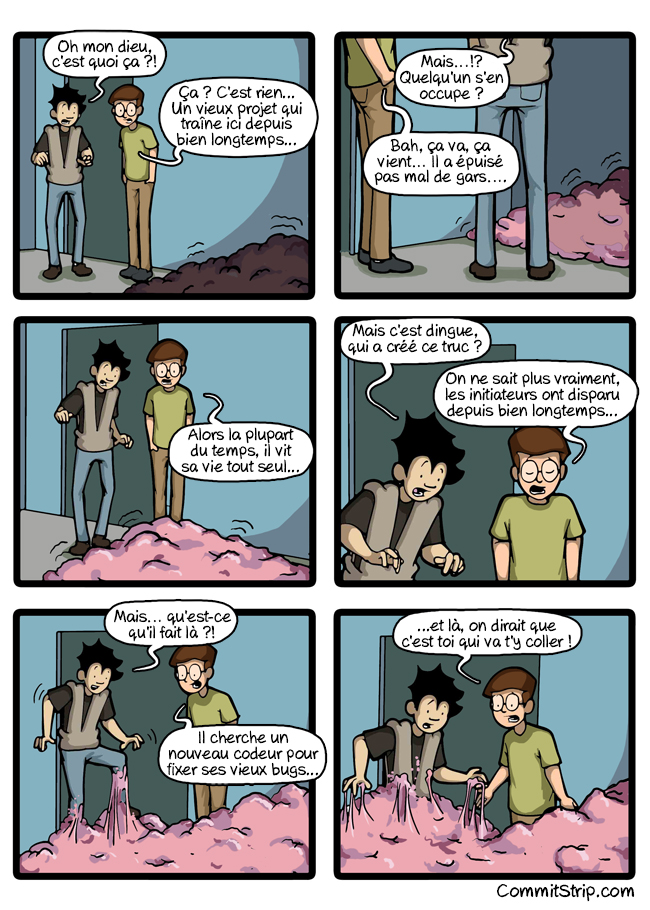
\includegraphics[width=0.45\textwidth]{assets/blob.jpg}
\caption{Illustration de la dette technique}
\label{fig:my_label}
\end{figure}

\newpage

\section{Pourquoi le pilotage de la qualité}

Plus que jamais, s’appuyer sur des infrastructures informatiques pérennes et robustes constitue un élément stratégique pour les entreprises. 
On constate pourtant que beaucoup d’entreprises déplorent une qualité médiocre des développements réalisés et investissent des sommes considérables pour pallier à cette problématique. Ce constat est particulièrement évident lorsque qu’il s’agit d’une application stratégique, pouvant impacter fortement les performances ou la qualité de service d’une entreprise.


\subsection{La théorie}

Le pilotage de la qualité est un aspect incontournable du développement. 
C'est un processus complexe qui doit être mené dès le début du cycle de développement du projet afin de porter ses fruits. 

Le pilotage de la qualité doit prendre en considération plusieurs paramètres pour être efficace : 

\begin{description}
\item[Paramètres technologiques]{où le logiciel doit être maintenable, fiable, évolutif, sécurisé,
transferable proposant ainsi une infrastructure informatique pérenne et robuste.} 
\item[Paramètres organisationnels]{et relatif à la gestion de projet, permettant d'appliquer les bonnes pratiques tout au long du développement du logiciel.} 
\end{description}

\newpage

Lorsque ces deux aspects sont en synergie, ils permettent de garantir un pilotage efficace. 
En effectuant une conduite de la qualité de manière continue cela permet de prévenir beaucoup d'erreurs en amont de la sortie du logiciel et permettre de limiter l'impact technique et financier. 
De manière plus générale, cet aspect qualitatif, doit permettre aux entreprises de structurer leur approche du développement en mettant en place des règles strictes pour tout nouveau projet. 

Le pilotage de la qualité doit également être intuitif et lisible par les différentes populations de l'entreprise et ne doit donc pas être uniquement réservé aux développeurs. 
A l'aide de tableaux de bords proposant une vision claire et précise du projet pour permettre alors de partager la situation avec tous les acteurs du projet. 

\section{Pilotage de la qualité dans la pratique}

Le paragraphe précédent, aborde le pilotage de la qualité d'un point de vue théorique, mais comment mettre en place ces préceptes de manière simple et efficace dans la pratique?

\section{Conception}

La phase de conception du logiciel est tout aussi importante voir même plus importante que la phase d'écriture du code. 
Les développeurs se doivent de réfléchir à tous les aspects du logiciel en amont. 
Plusieurs méthodes permettent d'être efficace sur ce point. 

\subsubsection{User story}
Les user story ou récit d'utilisateur en français sont des phrases simple dans le langage naturel permettant de décrire avec suffisamment de précision le contenu d'une fonctionnalité à développer. 

La phrase contient généralement trois élements descriptifs de la fonctionnalité : Qui ? Quoi ? Pourquoi ? 

\paragraph{Exemple}

\begin{verbatim}
En tant qu'utilisateur
je veux pouvoir rechercher mes clients par leur prénom et leur nom de famille afin de les
retrouver rapidements lorque je reçois un appel de leur part. 

En tant qu'utilisateur,
je veux pouvoir modifier mes emplois du temps mais pas ceux des autres utilisateurs
\end{verbatim}

\subsubsection{Use case}
Les use cases ou cas d'utilisation, représente une interaction possible entre un utilisateur et le système. 

La rédaction des cas d'utilisations passe par des diagrammes d'utilisation. 

Les utilisateurs sont appelés acteurs et ils interagissent dans les cas d'utilisations.


\begin{figure}[h!]
\centering
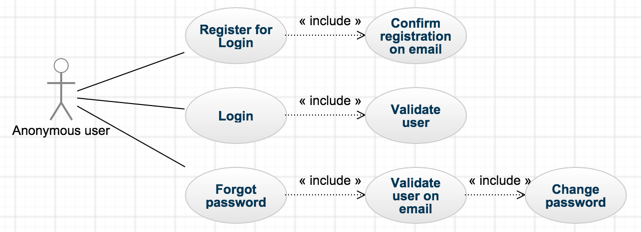
\includegraphics[width=1\textwidth]{assets/use_case_exemple.png}
\caption{Exemple d'un diagramme de cas d'utilisation}
\label{fig:my_label}
\end{figure}

\newpage

\subsubsection{Diagramme d'activité}

Permettant de représenter le déclenchement d'événements en fonction des états du système.
Il peut être également utilisé pour décrire un flux de travail. 

\begin{figure}[h!]
\centering
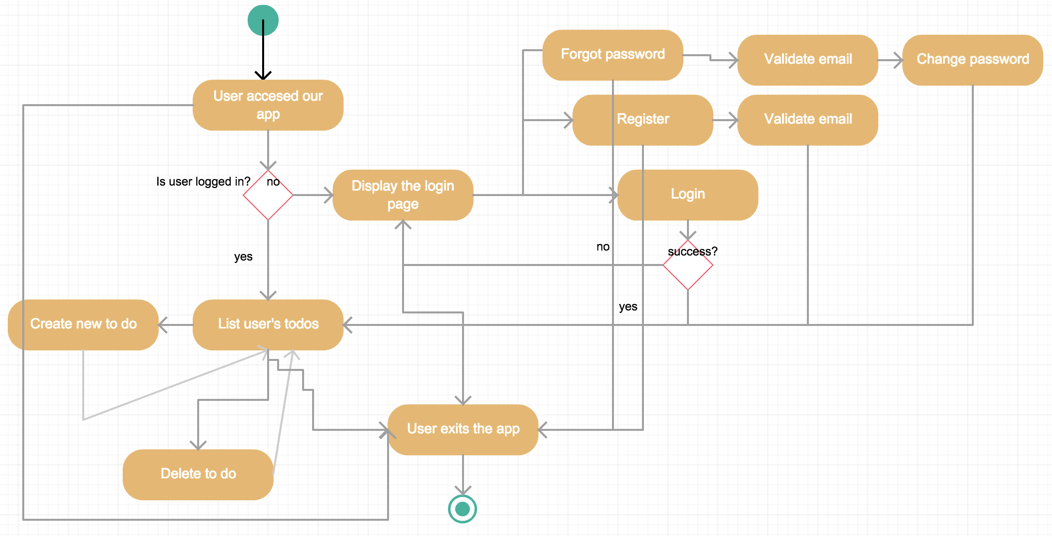
\includegraphics[width=1\textwidth]{assets/activity_diagram.png}
\caption{Exemple d'un diagramme de cas d'utilisation pour un gestionnaire des tâches}
\label{fig:my_label}
\end{figure}

Ce diagramme sera particulièrement utile pour définir les différents chemins qu'un utilisateur peut prendre dans notre application et donc définir ceux qu'ils ne peut pas prendre et mettre en place les routines de sécurité en conséquence. 

\paragraph{Exemple des activités exprimées dans le diagramme ci-dessus}
\begin{verbatim}
- Un utilisateur accede à notre gestionnaire des tâches 
- Si l'utilisateur n'est pas connecté, il verra la page de connection.
- Si l'utilisateur a déjà un compte, il peut se connecter
- Si l'utilisateur a un compte mais a oublié son mot de passe, il peut récupérer son mot de passe
- Si l'utilisateur n'a pas de compte, il peut en créer un. 
- Les deux actions, créer un compte et récupérer mon mot de passe nécessitent une validation d'email. Un utilisateur peut se connecter à l'application, uniquement après que son adresse email ait été confirmé. 
- Si l'utilisateur est déjà connecté, il verra son gestionnaire des tâches (qui peut être vide si il ne contient pas de tâches). 
- Lorsqu'il est connecté l'utilisateur peut 
  - voir sa liste des tâches
  - marquer une tâche comme effectuée
  - rechercher dans sa liste des tâches
  - supprimer une tâche d'une liste
  - se déconnecter
- L'utilisateur peut se déconnecter à tout moment 
\end{verbatim}



\section{Tests}
Un test désigne une procédure permettant de vérifier partiellement un système. 

\subsubsection{Objectif}
L'objectif premier des tests est d'identifier les comportements problématiques du logiciel pour en augmenter la qualité. 

\subsubsection{Classification des tests}

\begin{figure}[h!]
\centering
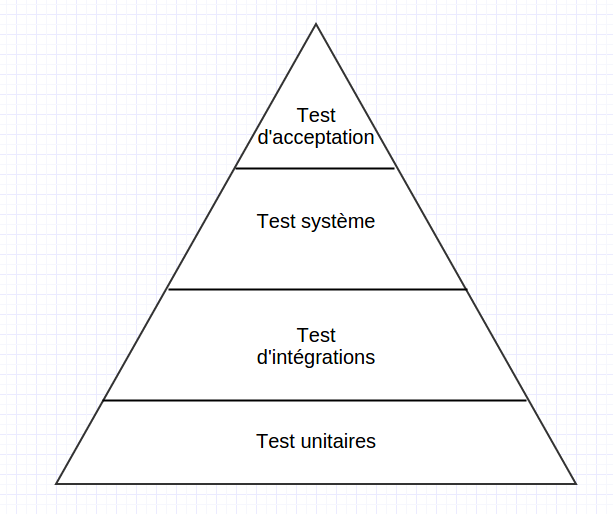
\includegraphics[width=0.7\textwidth]{assets/pyramide_tests.png}
\caption{Quatres niveaux de test}
\label{fig:my_label}
\end{figure}

Chaque test supérieur, dépend du test de niveau inférieur. 
Ainsi si les tests d'intégration ne fonctionnent pas, les tests système ne s'executeront pas. 


\subsection{Test unitaires}
Les tests unitaires sont des procédures permettant de vérifier le bon fonctionnement d'une partie précise d'un logiciel ou d'un module d'un programme. 

\subsubsection{Utilité}
Ils permettent d'assurer que la spécification correspondante à la partie du logiciel testée est bel est bien réalisée. 


\begin{description}
    \item Ils permettent également de trouver rapidement les erreurs 
    \item Ils permettent également de sécuriser la maintenance en signalent les éventuelles régressions du programme, en cas de modification. Certains tests peuvent échouer lorsqu'une nouvelle fonctionnalité est implémentée, il faut donc réécrire le test pour le faire correspondre aux nouvelles attentes, ou corriger l'erreur dans le code. 
    \item Les tests unitaires permettant enfin de documenter le code. En lisant un test unitaire, on va pouvoir comprendre très rapidement le fonctionnement d'une méthode. Il est possible que la documentation d'une application ne soit plus à jour, en revanche les tests eux correspondent à la réalité de l'application. 
\end{description}

Les tests unitaires sont aussi simples que possible, facilement "débugable", doivent être rapides à éxecuter

Voir l'annexe, pour un exemple de test unitaire. 
% Annexe emple de test unitaire


\subsection{Test d'intégration}
Les tests d'intégration chacun des modules indépendants du logiciel sont assemblés et testés dans l'ensemble. 

\subsubsection{Objectifs}
L'objectif est de détecter les erreurs qui n'ont pas pu être détectées lors des tests unitaires. 

Ces tests permettent également de vérifier l'aspect fonctionnel du logiciel ainsi que ses performances et sa fiabilité. 

La particularité des tests d'intégration est l'environnement.
En effet, les tests unitaires vont être executés dans l'ensemble effectuant différentes actions (requêter une base de donnée, consumer un service REST, etc), et ceux dans différents environnement pour s'assurer que les différents environnement n'affectent pas le comportement du code. 

\subsection{Test système}
Les test système permettent d'évaluer la conformité du système face aux exigences spécifiées.

Ces tests vérifient la conception mais également le comportement et les attentes présumées du client. 


\subsection{Test d'acceptation}
C'est le dernier niveau de test, on l'appelle également recette. 

Ce test vise à assurer de manière formelle que le produit complet est conforme aux spécifications. 

\paragraph{Exemple de tests d'acceptation}

\begin{verbatim}
- Cliquer sur le bouton de zoom, doit élargir le document de 25%
\end{verbatim}

L'avantage de ces tests et qu'ils sont écrit en langage naturel (français par exemple) et s'assure que l'ensemble des fonctionnalités du logiciel fonctionne. 
Cependant les tests d'acceptation peuvent s'avérer particulièrement difficile à débuger, car ils se basent sur beaucoup de lignes de code. 

Egalement, en méthodologie agile, les test d'acceptation sont censés être le miroir des user stories (vu précédemment). 
Si les tests passent, ça signifie que la user story rejoint les besoins du client et que cette récit utilisateur est complet. 

% Ajouter la documentation. 

\subsubsection{Conclusion}

Tous ces tests sont complémentaires. Parfois il est préférable de se concentrer sur un type de test ou d'en éviter d'autres.
La principale différence entre ces différents niveaux de test, réside dans le fait que certains tests sont destinés au développeur, tandis que d'autres aux attentes clients. 

\section{Usine logiciel}
L'intégration d'un projet est constituée de différentes étapes souvent laborieuses et consommatrices de temps. Parmi ces étapes, nous retrouvons généralement les phases de génération de code, de compilation, l'exécution d'outils de qualité de code, l'exécution d'outils de tests unitaires et fonctionnels, de génération de code, des phases de validation et de vérification d'éléments transverses comme les licences, de déploiement, ...
\jumpOne
Cette phase d'intégration est d'autant plus critique qu'elle est faite en fin de projet avant la livraison, et que révélant de nombreux problèmes elle risque de mettre la réussite du projet en péril.
\jumpOne
L'ensemble de ces problèmes sont supprimés avec la mise en place de l'intégration continue qui va constiter à mettre en place un ensemble d'outils pour automatiser le processus d'intégration. Celui-ci est exécuté à chaque changement dans l'environnement d'infrastructure du projet et produit un ensemble de résultats que les membres de l'équipe de développement puissent visualiser à chaque instant.

\subsection{Intégration continue}
L'intégration continue est une pratique visant à vérifier qu'à chaque modification du code d'un logiciel, il ne se produit pas de régression sur ce logiciel. 

L'intégration est utilisée à l'aide d'une plateforme d'intégration continue (comme Jenkins).

Cette plateforme va permettre aux développeurs de pouvoir déployer leurs applications, d'une manière automatisée et industrielle en validant un certain nombre de règles que le projet doit respecter pour être mis en production.
\jumpOne
A chaque modification du code (généralement provoqué par un \gls{commit}
d'un des developpeurs, un processus est lancé et va executer tous les tests unitaires et fonctionnels. 
En plus d'éxecuter les tests, généralement une analyse statique du code est effectuée, permet de déterminer la qualité du code en lui même. 

\begin{itemize}
\item Détection rapide d'une anomalie logicielle et diminution du coût tardif d'une correction logicielle
\item Cohésion de l'équipe de développement
\item Automatisation des tests
\item Suivi de la qualité du code logiciel
\item Visibilité dans l'avancement du projet
\item Version déployée et disponible en continue
\item Automatisation de la livraison
\end{itemize}

\begin{figure}[h!]
\centering
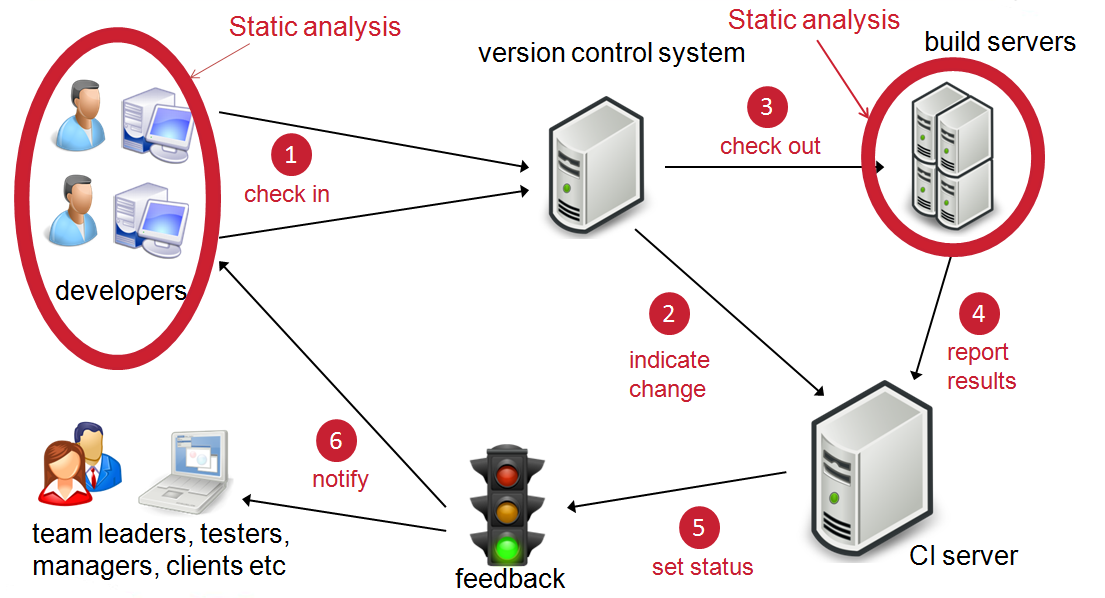
\includegraphics[width=0.7\textwidth]{assets/ci.png}
\caption{Intégration continue}
\label{fig:my_label}
\end{figure}

\paragraph{Explication}
\begin{enumerate}
\item Les développeurs publient leurs modifications au système de versionning
\item Ce système indique au gestionnaire d'intégration continue un chargement
\item Les tests sont exécutés ainsi que l'analyse statique du code
\item Le serveur d'intégration continue rapporte par la suite aux développeurs et au management l'état du projet après les modifications.
\end{enumerate}

\section{Revue de code}
La revue de code est un autre moyen d'identifier des bugs. 
Il consiste à faire une revue du code source développée par un développeur expérimenté. 

La mise en place de revue de code, de manière systématique pendant la phase de développement permet de responsabiliser les développeurs car, le travail de chacun sera systématiquement évalué par quelqu'un d'autre. 

Ce système va permettre d'améliorer la qualité du code écrit. De plus le relecteur pourra identifier des bugs ou des axes d'amélioration possible. 

Il existe trois processus de revue de code 

\begin{enumerate}
    \item Revue de code bloquante : Tout développement doit être relu avant d'être commité sur le \gls{depot} 
    A comme inconvénient de freiner le développement, car certains développements peuvent se retrouver en attente d'une relecture dont ils dépendent. 
    \item Revue de code non-bloquante : Tout développement commité sur le dépôt doit être relu. 
    Permet de laisser les développeurs continuer à travailler sans relecture. 
    \item Revue de code avec développement par binôme : faite en permanence par le même binôme. 
    Cependant le travail en binôme influence le jugement du relecteur direct. 
\end{enumerate}

La revue de code non-bloquante semble être la meilleure méthode. D'autant plus qu'il existe des produits et des plugins pour les \gls{IDE} 
permettant de gérer ces revues facilement. 

\newpage

\section{Documentation}
Un élement important et beaucoup négligé est la documentation du développement. 
Cependant, un développeur est souvent amené à régulièrement travailler sur de nouveaux projets où les choix techniques varient beaucoup, où l'on doit comprendre l’existant et répondre à la question “comment en est-on arrivé là ?” avant de pouvoir critiquer et de faire un état des lieux adapté.

Il existe trois types de documentation, chacune servant son propos, plus difficile étant d’estimer comment les tenir à jour :


\begin{description}
    \item[Doc technique]
    {explique comment et surtout pourquoi ça fonctionne. Cette documentation est la plus simple à mettre en place, c'est celle qui est directement dans le code.}
    \item[Doc des choix techniques]
    { Ce type de documentation est souvent peu employée. Au-delà de la valeur des choix effectués, il est très intéressant de savoir pourquoi ces choix ont étés faits, et les conséquences positives et négatives envisagées. Cela permet, une fois en situation plus difficile, de s’en remettre aux explications de l’époque, et de vérifier qu’elles soient toujours justifiées et d’actualité.
        
    }
    \item[Doc métier]{C'est la vision du maitre d'ouvrage, définissant le périmètre fonctionnel, etc. }
\end{description}

Les deux idées maîtresses autour de la documentation sont, d’une part qu’il est préférable de documenter le pourquoi plutôt que le comment, et d’autre part que bien que la documentation soit nécessaire, il faut documenter suffisamment mais pas trop ; c’est dans cet équilibre que réside toute la difficulté. Autrement, la documentation peut devenir une dette à elle toute seule.

\newpage


\section{Adapter la méthode gestion de projet aux bonne pratiques}
Enfin, pour que toutes ces bonnes pratiques puissent pleinement s'intégrer dans le cycle de développement de logiciel, il est nécessaire d'adapter la méthode de gestion de projet et les pratiques qui en découlent. 

Plusieurs questions se posent.

\begin{itemize}
\item Quelles méthodes choisir ?
\item Comment les mettre en place ? 
\end{itemize}

Le prochain chapitre sera consacré à la méthode phare qui est utilisé pour intégrer ces bonnes pratiques de développement, \textbf{l'agilité} et en particulier le \textbf{scrum}. 

\begin{figure}[h!]
\centering
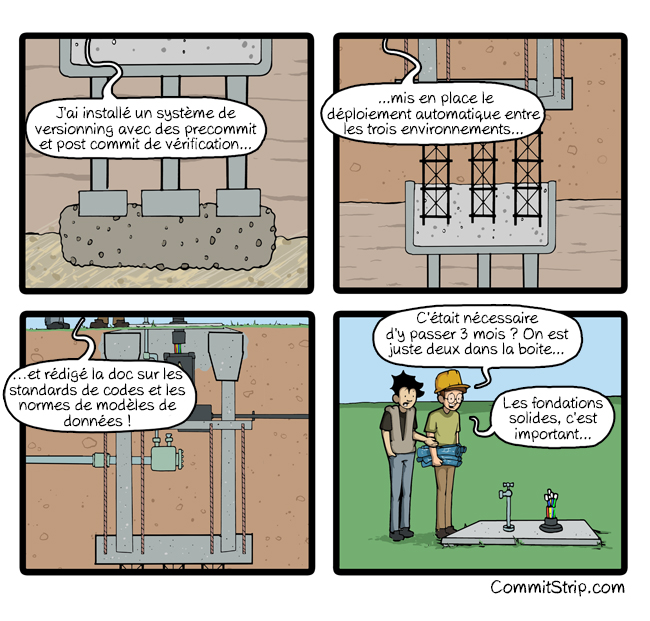
\includegraphics[width=0.8\textwidth]{assets/foundation.jpg}
\caption{Métaphore des bonnes pratiques de développement}
\label{fig:my_label}
\end{figure}
    
    \chapter{Agilité et Scrum}

\section{Méthodes Agiles}

\subsection{Présentation}
Les méthodes de développement dites "méthodes agiles" (en anglais Agile Modeling) visent à réduire le cycle de vie du logiciel (donc accélérer son développement) en développant une version minimale, puis en intégrant les fonctionnalités par un processus itératif basé sur une écoute client et des tests tout au long du cycle de développement. 

L'origine des méthodes agiles est liée à l'instabilité de l'environnement technologique et au fait que le client est souvent dans l'incapacité de définir ses besoins de manière exhaustive dès le début du projet. Le terme "agile " fait ainsi référence à la capacité d'adaptation aux changements de contexte et aux modifications de spécifications intervenant pendant le processus de développement. 

\subsection{Principes et fonctionnement de la méthode Agile}

Le principe de base des méthodes "Agile" est qu’il est contre-productif de développer un produit, en planifiant et en spécifiant les moindres détails. 
En effet, prévoir tous les aspects de la production entraîne dans la plupart des cas frustrations et pertes de temps car les aléas surviennent fréquemment. C’est cette approche prédictive et séquentielle de type cascade ou cycle en V que les tenants des méthodes "Agile " veulent casser. Ainsi, au lieu de fixer les objectifs lointains, le mieux serait de procéder par étapes c’est-à-dire fixer des objectifs à court terme et commencer le développement sans perdre de temps. Chaque fois que cet objectif est atteint, on passe au prochain et ainsi de suite jusqu’à atteindre le but ultime. Au niveau d’un développement de logiciel, c’est le client qui transmet à l’équipe de développeurs sa vision du produit avec la liste des fonctionnalités qu’aurait ce produit. Il communique ainsi directement avec l’équipe et ensemble ils estiment le coût de chaque fonctionnalité pour aboutir à une idée approximative du budget final. De ce fait, on raisonne plus "produit" que "projet", d’où l’utilisation du terme "gestion de produit" au lieu de "gestion de projet".

\subsection{Valeurs fondamentales}
4 valeurs fondamentales provenant du manifeste Agile. 

\begin{enumerate}
\item \textbf{L'équipe} ("Les individus et leurs interactions, plus que les processus et les outils") : dans l'optique agile, l'équipe est bien plus importante que les outils (structurants ou de contrôle) ou les procédures de fonctionnement. Il est préférable d'avoir une équipe soudée et qui communique, composée de développeurs (éventuellement à niveaux variables), plutôt qu'une équipe composée d'experts fonctionnant chacun de manière isolée. La communication est une notion fondamentale.
\item \textbf{L'application} ("Des logiciels opérationnels, plus qu'une documentation exhaustive ") : il est vital que l'application fonctionne. Le reste, et notamment la documentation technique, est une aide précieuse mais non un but en soi. Une documentation précise est utile comme moyen de communication. La documentation représente une charge de travail importante, mais peut pourtant être néfaste si elle n'est pas à jour. Il est préférable de commenter abondamment le code lui-même, et surtout de transférer les compétences au sein de l'équipe (on en revient à l'importance de la communication).
\item \textbf{La collaboration} ("La collaboration avec les clients, plus que la négociation contractuelle ") : le client doit être impliqué dans le développement. On ne peut se contenter de négocier un contrat au début du projet, puis de négliger les demandes du client. Le client doit collaborer avec l'équipe et fournir un compte rendu continu sur l'adéquation du logiciel avec ses attentes.
\item \textbf{L'acceptation du changement} ("L'adaptation au changement, plus que le suivi d'un plan") : la planification initiale et la structure du logiciel doivent être flexibles afin de permettre l'évolution de la demande du client tout au long du projet. Les premières livraisons du logiciel vont souvent provoquer des demandes d'évolution.
\end{enumerate}

\subsection{Principes généraux}

Ces quatres valeurs se déclinent en 12 principes généraux communs à toutes les méthodes agiles. 
\begin{enumerate}
    \item  La plus haute priorité est de satisfaire le client en livrant rapidement et régulièrement des fonctionnalités à forte valeur ajoutée.
    \item Le changement est accepté, même tardivement dans le développement, car les processus agiles exploitent le changement comme avantage concurrentiel pour le client.
    \item La livraison concerne une application fonctionnelle, toutes les deux semaines à deux mois, avec une préférence pour la période la plus courte.
    \item Le métier et les développeurs doivent collaborer régulièrement et de préférence quotidiennement au projet.
    \item Le projet doit impliquer des personnes motivées. Donnez-leur l'environnement et le soutien dont elles ont besoin et faites leur confiance quant au respect des objectifs.
    \item La méthode la plus efficace pour transmettre l'information est une conversation en face à face.
    \item L’unité de mesure de la progression du projet est un logiciel fonctionnel (ce qui exclut de comptabiliser les fonctions non formellement achevées).
    \item Les processus agiles promeuvent un rythme de développement soutenable (afin d’éviter la non qualité découlant de la fatigue).
    \item Les processus agiles recommandent une attention continue à l'excellence technique et à la qualité de la conception.
    \item La simplicité et l'art de minimiser les tâches parasites, sont appliqués comme principes essentiels.
    \item Les équipes s'auto-organisent afin de faire émerger les meilleures architectures, spécifications et conceptions.
    \item À intervalle régulier, l'équipe réfléchit aux moyens de devenir plus efficace, puis accorde et ajuste son processus de travail en conséquence.
\end{enumerate}


\section{Scrum}

Scrum est un schéma d’organisation de développement de produits complexes. Il est défini par ses créateurs comme un "cadre de travail permettant de répondre à des problèmes complexes et changeants tout en livrant de manière productive et créative des produits de la plus grande valeur possible ". Scrum est considéré comme une méthode agile.
\jumpOne
La méthode s'appuie sur le découpage d'un projet en boîtes de temps, nommés "sprints ". Les sprints peuvent durer entre quelques heures et un mois (avec une préférence pour deux semaines). Chaque sprint commence par une estimation suivie d'une planification opérationnelle. Le sprint se termine par une démonstration de ce qui a été achevé. Avant de démarrer un nouveau sprint, l'équipe réalise une rétrospective. Cette technique analyse le déroulement du sprint achevé, afin d'améliorer ses pratiques. L'adaptation et la réactivité de l'équipe de développement est facilitée par son auto-organisation.


\subsection{Fonctionnement du Scrum}

\subsubsection{Piliers du scrum}

\begin{enumerate}
\item \textbf{La transparence} : Scrum met l'accent sur le fait d'avoir un langage commun entre l'équipe et le management. Ce langage commun doit permettre à tout observateur d'obtenir rapidement une bonne compréhension du projet.
\item \textbf{L'inspection }: À intervalle régulier, Scrum propose de faire le point sur les différents artéfacts produits, afin de détecter toute variation indésirable.

Ces inspections ne doivent pas être faites trop fréquemment, ou par un inspecteur mal formé : cela nuirait à l'avancement du projet.
\item \textbf{L'adaptation} : Si une dérive est constatée pendant l'inspection, le processus doit alors être adapté. Scrum fournit des rituels, durant lesquels cette adaptation est possible. Il s'agit de la réunion de planification de sprint, de la mêlée quotidienne, de la revue de sprint ainsi que de la rétrospective de sprint.
\end{enumerate}

\subsection{Caractéristiques}

Le framework Scrum consiste en la définition des rôles projets, activités ou artefacts, et réunions ou événements.

\subsubsection{Rôles}
Scrum définit trois rôles : \textit{Product Owner}, \textit{le Scrum Master} et le \textit{Développeur}. Il est à noter que le rôle de développeur couvre plusieurs métiers d'une organisation traditionnelle.

\begin{description}
    \item \textbf{Product Owner} est le représentant des clients et des utilisateurs. Il est "responsable de maximiser la valeur du produit et du travail de l'équipe de développement".  Il est seul à diriger l'activité de l'équipe de développement. 
    
    Par conséquent, cet acteur se charge de différents "sous-rôles" et à plusieurs responsabilités 
    \begin{itemize}
    \item Il explicite les éléments (Items) du Carnet du produit.
    \item C'est lui qui définit l'ordre dans lequel les fonctionnalités seront développées. Il prend les décisions importantes concernant l'orientation du projet.
    \item Il s'assure que le carnet du produit est visible et compris de l'équipe de développement.
    \end{itemize}
    
    C'est également lui qui, en accord avec l'équipe, fixe les objectifs d'un incrément (Sprint) au début de celui-ci. Si ces objectifs deviennent obsolètes pendant le sprint, il a alors la possibilité d'interrompre le sprint en cours.

Dans l'idéal, travaille dans la même pièce que l'équipe. Il est important qu'il reste très disponible pour répondre aux questions de l'équipe et pour lui donner son avis sur divers aspects du logiciel.

    \newpage
    
    \item \textbf{Scrum master} : Il aide le groupe à apprendre et à appliquer le Scrum afin que la valeur métier se
matérialise. Le ScrumMaster fait tout ce qui est en son pouvoir pour aider l’equipe, le product
owner et l’organisation à réussir le projet. Il n’est pas le manager de l’Equipe, ni
même un chef de projet, un chef d’équipe ou un représentant de l’equipe. Son rôle est plutôt de
servir l’equipe; il aide à supprimer les obstacles, protège les développeurs des interférences extérieures, et
facilite l’adoption par les développeurs des pratiques modernes du développement. 

Il enseigne, il coache et guide le Product Owner, les développeurs ainsi que le reste de l’organisation dans une utilisation fine de Scrum. Il s’assure que chacun (y compris le Product Owner, ainsi que le top management) comprenne les principes et les pratiques de Scrum, et il accompagne l’organisation dans le changement souvent difficile mais nécessaire au succès du développement agile. 

Etant donné que Scrum met en lumière les obstacles et les menaces qui pèsent sur l’efficacité des développeurs et du Product Owner, 
il est important d’avoir un Scrum Master engagé et travaillant énergiquement à la résolution des problèmes auxquels seront confrontés aussi bien l’équipe que le Product Owner. 
Il y a idéalement un ScrumMaster dédié et à plein temps, bien qu’une petite équipe puisse voir l’un de ses membres jouer ce rôle (on réduit alors sa charge sur les travaux courants).  
    \item \textbf{L'équipe de développement, les développeurs}. construit le produit qui est défini par le Product Owner : une application ou un site web par exemple. 

Dans Scrum, l’Equipe est "plurifonctionnelle" : elle inclut toute l’expertise nécessaire pour fournir une version du produit potentiellement livrable à chaque Sprint. 

Elle est également "auto organisée" (autogérée), avec un grand degré d’autonomie et de responsabilité. L’équipe décide des éléments à implémenter dans un Sprint (éléments issus de la liste proposée par le Product Owner), et des moyens les plus adaptés pour réaliser cet objectif.

Chaque personne dans l’Equipe est simplement qualifiée de membre. Il faut noter qu’il n’y a pas de
titre de spécialiste au sein d’un groupe qui adopte Scrum; pas d’analyste fonctionnel, pas de DBA,
pas d’architecte, pas de team leader, pas de concepteur IHM, pas de programmeur. 


Tous les membres travaillent ensemble durant chaque Sprint, par tous les moyens appropriés et 
nécessaires à l’atteinte de l’objectif qu’ils ont eux-mêmes déterminé.

Etant donné qu’il n’y a que des membres, l’Equipe n’est pas seulement pluridisciplinaire mais fait
également preuve de capacité diverse d’apprentissage; chacun possède certainement des atouts
particuliers, mais continue également de progresser sur d’autres spécialités. 

Chaque personne devra posséder des compétences sur différents domaines et à différents niveaux, et devra "aller là où le travail se trouve". Les individus doivent être à même de prendre en charge des tâches dans des
domaines moins familiers lorsqu’il est nécessaire de faciliter la finalisation d’un élément. 

 Dans Scrum, les Equipes sont plus productives et efficaces si tous les membres sont
dédiés à 100\% à un seul produit au cours d’un Sprint. Afin d’éviter des changements de contextes et
un fléchissement dans la focalisation, inconvénients souvent coûteux, il faut éviter la multiplication
des tâches entre plusieurs projets ou produits. Les équipes stables étant plus productives, il faut
éviter les changements au sein de l’équipe.

\end{description}

\newpage

\subsubsection{Scrum Master et Product Owner ne peuvent être la même personne}

Le scrum master et le product owner, ne peuvent pas être la même personne tant leurs objectifs sont différents et la combinaison des deux rôles conduits souvent à la de la congusion et des conflits. 
En effet cette combinaison va pousser le PO à faire du micro management, ce qui est à l'opposé des équipes auto-organisées telles que Scrum le définit. 
A la différence d'un manager classique, le scrum master ne dit pas à chacun ce qu'il doit faire et n'assigne pas de tâches. Il facilite le processus en soutenant les développeurs dans son organisation et sa gestion. Si le scrum master était précédemment en position de chef de projet au sein des développeurs, il devra changer significattivement d'état d'esprit pour que les développers puissent pleinement profiter du scrum. 

\subsubsection{Scrum sans chef de projet ?}

On pourra noter qu'il n'existe pas de chef de projet dans la méthologie scrum. En réalité il n'est pas nécessaire. 
Les responsabilités traditionnellement associées au chef de projet ont été divisées et réassignées aux trois rôles de scrum et principalement aux développeurs et au product owner, plutôt qu'au scrum master. 
Pratiquer le scrum en y ajoutant un chef de projet indique une méconnaissance fondamentale de scrum et conduit typiquement à des conflits dans les reponsabilités, un manque de clarté dans l'autorité et au final de piètres résultats. 
Parfois un ancien chef de projet peut jouer le rôle de scrum master, mais la réussite de cette approche est largement dépendante des individus et de la façon dont ils comprennent les différences fondamentales entre ces deux positions.

\subsubsection{Adaptation des autres acteurs du projet au Scrum}

En plus des trois rôles, d'autres parties prenantes contribuent au succès du projet. Parmi elles, les manager, clients et les utilisateurs. 
Certaines parties prenants, telles que les directions fonctionnelles ou techniques pourront voir évoluer significativement leurs rôles dans une organisation adoptant le Scrum, mais ils gardent néanmoins toute leur valeur. 

\begin{itemize}
    \item Ils soutiennent l'équipe en respectant les règles et l'esprit de scrum
    \item Ils aident à supprimer les obstacles que l'équipe et le product owner identifient
    \item Ils fournissent leur expertise et leur expérience. 
\end{itemize}

Ainsi ces personnes ne sont plus considérés comme des micro-manager (assignant des tâches, obtenant l'état d'avancement, etc) mais deviennent les véritables serviteurs de l'équipe de développement. 
Par le biais de conseils, coaching, facilitant la suppression des obstacles et la résolution des problèmes, fournissant des idées créatives, et apportant leurs compétences aux membres de l'équipe de développeurs.


\section{Artéfact du scrum}

\subsection{Product Backlog}

Lorsqu'une entreprise décide d'utiliser Scrum sur un projet, avant même de pouvoir démarrer le premier sprint elle a besoin d'un \textbf{product backlog} ou \textbf{carnet de produit}, correspondant à une liste priorisée (ordonnée) des caractéristiques orientées client. 

C'est l'unique source des besoins pour tous les changements à effectuer sur le produit. 
Le product backlog est un document qui évolue constamment au cours de la vie du produit et n'est jamais réellement terminé. 

Il n'existe qu'un seul product backlog pour un produit. 

\subsubsection{Contenu}

Ce carnet de produit, va contenir une variété d'élements : 

\begin{itemize}
\item \textbf{Nouvelles fonctionnalités métier}, possibilité pour chaque utilisateur d'ajouter un article au panier
\item \textbf{Objectifs majeurs d'ingénierie}, réécrire le système PHP en Java
\item \textbf{Améliorations technique}, refonte du module de transactions afin de le rendre plus extensible
\item \textbf{Travaux exploratoires}, étudier une solution de stockage plus rapide que celle actuelle
\item A\textbf{nomalie connu du système}\footnote{
Les anomalies sont dans le product backlog dans le cas ou elles sont peu nombreuses. }, diagnostiquer et corriger l'erreur dans le script de traitement des commandes. 
\end{itemize}


Tout ces éléments, sont élaborés de différentes manières à partir du moment ou ils restent clairs et viables sur la durée du projet. 


\begin{figure}[h!]
\centering
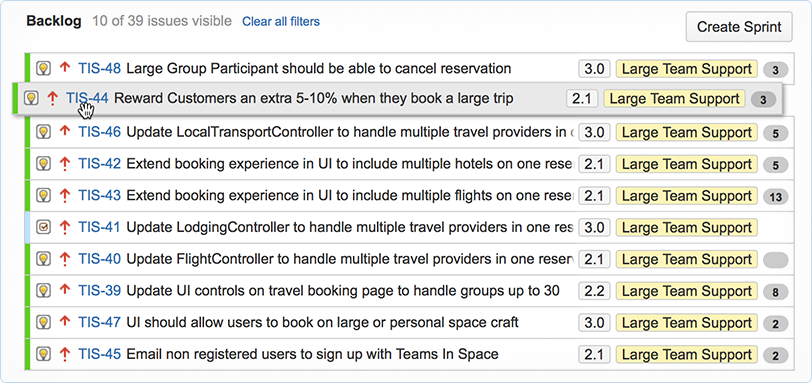
\includegraphics[width=1\textwidth]{assets/product_backlog.png}
\caption{Exemple d'un product backlog sur le logiciel JIRA, contenant plusieurs tâches}
\label{fig:my_label}
\end{figure}

Chaque élement du product backlog doit être : 

\begin{description}
    \item[Détaillé]{Les éléments les plus prioritaires sont de granularité plus fine et sont plus détaillés que les autres.}
    \item[Estimé]{Chaque élement doit être estimé au préalable et peut être réestimé à chaque sprint, en fonction des nouvelles informations apparues et de la connaissance acquise. A chaque début de sprint, l'équipe fournit au product owner, une estimation de l'effort requis pour chaque élément du product backlog et des risques techniques éventuels. }
    \item[Flexible]{Du fait de la nature du scrum, le product backlog est affiné régulièrement. Les élements peuvent être modifiés, ajoutés, supprimés à chaque sprint. Ainsi le Product Backlog est continuellement mis à jour par le product owner afin de refléter les évolutions du besoin client, les nouvelles idées ou enseignements, les mouvements de la concurrence, les obstacles techniques qui apparaissent, etc.}
    \item[Priorisé]{Les élements sont ordonnés par ordre de point d'effort. En général les élements plus prioritaires doivent être "rentable". Une plus grande valeur métier pour un moindre coût. L'augmentation de la priorité d'un élement peut également être motivée par la nécessité de s'attaquer aux risques importants, avant qu'ils n'apparaissent.}
\end{description}

L'estimation de élements permet d'avoir de manière approximative une projection dans le temps d'une potentielle date de release incluant une certain nombre de fonctionnalité. 



\subsection{Sprint backlog}

A chaque début de Sprint, un but est décidé. Pour atteindre cet object, l'équipe de développement choisit lors de la réunion de planification de sprint quels élements du product backlog seront réalisés. 

Ces élements sont alors groupés dans un carnet de sprint.
Ainsi chaque personne de l'équipe met à jour régulièrement le carnet de sprint au cours de son activité, afin que celui-ci donne une vision la plus précise possible de ce que l'épique prévoit de réaliser pour atteindre les objectifs du sprint. Le carnet de sprint est sous la responsabilité de l'équipe et elle seule peut la modifier en cours d'itération. 

\begin{figure}[h!]
\centering
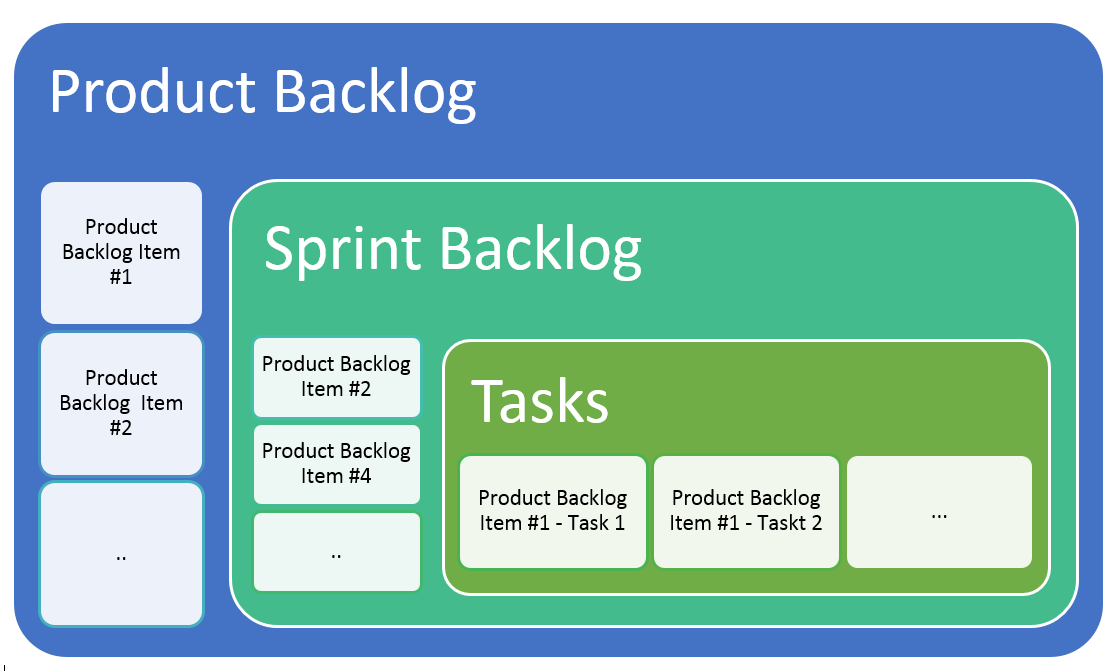
\includegraphics[width=0.7\textwidth]{assets/backlog.png}
\caption{Hiérarchie des backlog}
\label{fig:my_label}
\end{figure}


\subsection{Incrément de produit}

Chaque sprint, doit produire ce qui est officiellement appelé un incrément du produit, potentiellement livrable. 

C'est l'ensemble des des éléments du Sprint backlog finis pendant ce sprint et ceux pendant les sprint précédents. Les élements sont dits dans un état terminé lorsqu'ils remplissent leur rôle et qu'ils peuvent être utilisés directement. 

\section{Evénements}


\subsection{Sprint}
C'est l'évenement principal du scrum. C'est une période d'un mois maximum, durant laquelle l'équipe travaille et au bout duquel elle délivre un incrément du produit. 

La durée du Sprint est toujours la même durant tout le projet et un nouveau sprint démarre à chaque fois qu'un autre se termine. 



\begin{description}
    \item[Chaque sprint possède un but et sprint backlog]
    {
        Cependant, durant le sprint 
        
        \begin{itemize}
        \item l'objet ne peut être modifié
        \item la composition de l'équipe reste constante
        \item la qualité n'est pas négociable
        \item le sprint backlog est sujet à négociation entre le product owner et les développeurs. 
        \end{itemize}
    }
    \item[Limitation temporelle]
    {Un sprint peut durer au maximum un mois afin de limiter sa complexité et donc les risques liés au sprint. Chez Bob el web, la temps optimal est de 2 semaines
    }
    \item[Objet]
    {
        Si l'objet du sprint devient obsolète pendant celui-ci, le product owner peut décider de l'annuler en conséquence.  
        Ainsi les développements qui ont été terminés sont revus par le proriétaire du produit et peuvent être acceptés. 
        Ceux n'étant pas acceptés sont réestimés et remis dans le sprint backlog ce qui provoque le démarrage d'un nouveau sprint. 
    }
\end{description}



\subsection{Daily Scrum}

Dès que le sprint début, les développeurs se lancent quand une autre pratique fondamentale du scrum, le dail scrum (ou mêlée quotidienne en français). 
Il s'agit d'une courte réunion qui se déroule chaque jour de travail à heure fixe. Tout le monde y participe. 
Afin de garantirr que la réunion soit courte, il est nécessaire qu'elle se fasse en étant debout. 

C'est l'opportunité pour l'équipe de synchroniser ses travaux et d'échanger ensemble sur les obstacles recontrés ou à venir. 

Chaque membre de l'équipe expose successivement aux autres 3 points.

\begin{enumerate}
\item Qu'a-t-il fait depuis la dernière réunion ? 
\item Que va-t-il faire jusqu'à la prochaine réunion ? 
\item Quels sont les points d'obstacles ou de blocage rencontrés ou à prévoir ? 
\end{enumerate}


Il est important de noter que le daily scrum n'est pas une réunion de suivi pour le reporting à un manager. C'est au contraire le moment privilégié pour une équipe auto-organisé d'échanger sur la bonne marched l'activité et de se coordonner. 
En réalité pendant cette réunion, il n'y a presque pas de discussion et chacun doit juste répondre aux 3 questions. 
Si des discussions supplémentaires sont nécessaires, elles se tiennent lors de réunios consécutives, immédiatement après le daily scrum. 

Ces réunions sont un moyen supplémentaire d'inspection et d'adaptation. 


\subsection{Revue de Sprint}
Chaque fin de Sprint donne lieu à une revue de Sprint et une réunion de planification (préparant le prochain sprint). 

Cette réunion est prévue pour l'équipe et le product owner passent en revue le sprint qui vient de se terminer. 
Sont présents à cette réunion 

\begin{itemize}
\item L'équipe de développeurs
\item Le scrum master
\item Le product Owner
\item Les clients
\item Toute partie prenant, experts, décieurs et personnes intéressés. 
\end{itemize}

Chaque personne est libre de poser des questions ou d'apporter des contributions. 


L'objectif n'est pas réellement de faire une "démo" du travail accompli mais plutôt de regarder et d'étudier ce qu'il se passe et ainsi permettre de s'améliorer sur la base d'évaluations, en cycles itératifs. 
C'est également un excellent moyen pour le product owner de connaitre la situation actuelle du produit et de l'équipe de connaitre la situation actuelle du product owner du métier. 
Il est donc primordial qu'une conversation en profondeur s'établisse entre l'équipe et le product owner afin d'échanger sur la situation, obtenir des conseils, etc. 


\subsection{Réunion de préparation du prochain sprint}
A la suite de la revue de sprint, le product owner peut appliquer toute nouvelle mise à jour au product backlog. 
Il n'y a pas d'arrêt entre les sprints.

Par exemple, chez Bob el web les sprints durent 2 semaines, la revue de sprint s'effectue le vendredi matin et la préparation du prochain sprint le vendredi en début d'après midi après le daily scrum. 
\jumpOne
L'un des principes du développement agile est l'application d'un rythme soutenable, et c'est uniquement en travaillant aux heures normales et à une cadence raisonnable que les développeurs peuvent continuer ce cycle indéfiniment. 
La productivité des développeurs augment avec le temps grâce à l'évolution des pratiques et la suppression des obstacles qui ralentissent la cadence, et non pas en augmentant la charge de travail ou en faisant des compromis sur la qualité. 
\jumpTwo
Les sprints s'enchainent donc, jusqu'à ce que le product owner décide que le produit est prêt à être sorti. (Qu'une release sorte). 
Le summum du scrum, c'est qu'\textbf{un produit est potentiellement livrable à la fin de chaque sprint}, c'est à dire sans aucun travaux à terminer tels que des tests ou de la documentation.
Cela implique évidemment que tout soit complètement terminé à chaque Sprint, de telle sorte qu'il soit réellement possible de livrer le produit ou de le déployer immédiatement après la revue de sprint. 
\jumpOne
Cependant beaucoup d'organisations, possèdent des pratiques de développement, des outils et une infrastructure inadaptée et sont dans l'incapacité d'aboutir à cette vision de la perfection.
(On notera que les outils et l'infrastructure adapté est abordé dans la seconde partie de ce rapport). 


\begin{figure}[h!]
\centering
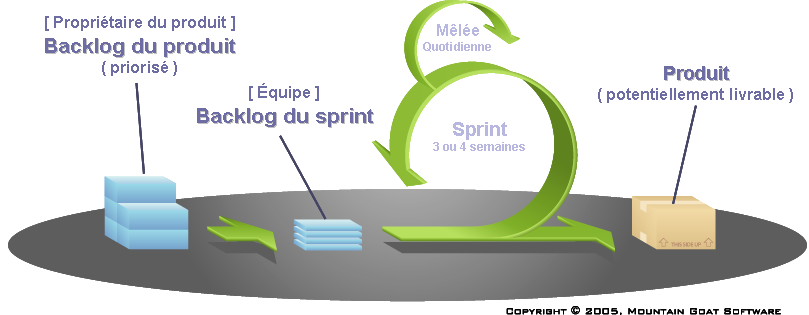
\includegraphics[width=0.8\textwidth]{assets/scrum.png}
\caption{Vue globale}
\label{fig:my_label}
\end{figure}

\newpage

\section{Développement de logiciel à travers la méthode agile chez Bob}
% Qu'est-ce qui était avant ? 
L'entreprise est passé d'une utilisation Agile light (avec seulement une liste de ticket à faire, au fur et a mesure) en Scrum il y'a plus d'un an. 

% Pourquoi Scrum ?
Le directeur technique de l'entreprise, Fred Wolf a pu aller voir le fonctionnement du scrum, par une équipe réelle par le biais d'un actionnaire. 
Le scrum est très adapté à Bob en raison du petit nombre de salariés.

% Av/In

D'un point de vue pratique et sur le terrain, le scrum permet chez Bob d'avoir une vision à moyen et court terme en se concentrant sur des tâches "éclatées", plutôt courtes et moyennement complexes. 

Cependant, le fait de changer souvent de tâches, voir de projet peut avoir des effets négatifs sur l'équipe de développeurs, qui doit constamment jongler entre plusieurs choses. 
Il est également plus difficile de donner des deadlines à long terme, puisqu'on avance par Sprint. 




% Montrer ici que le scrum était très intéressant 
% Depuis combien de temps êtes vous passés en mode Agile ?
%  on est passé en méthode Agile en mars 2014 (donc il y a un an et qq)
%- Vous utilisiez quoi avant ?
%avant on utilisait juste JIRA pour lister les tickets et on les faisait au fur et à mesure
%- Pourquoi avoir choisi l'agilité et le Scrum en particulier ?  Pour toi, quelles sont les avantages que l'agilité à apporter chez Bob?
%on a choisi Agile car cela nous permet de savoir où on va dans le temps tout en se concentrant sur des tâches relativement "atomiques" (donc plutôt courtes et moyennement complexes). Le Scrum en particulier je me souviens plus mais je crois qu'on a vite fait analyser les possibilités et c'était le plus approprié par rapport au nbre de personne chez BOB et à notre manière de travailler. En plus un de nos actionnaires gère une boîte qui fonctionne comme ça donc Fred a pu aller observer leur méthodologie avant de le mettre en place ici, mais on utilise de toute façon notre version du SCRUM qui n'est pas la version théorique mais une adaptation.
%- et les inconvénients ?
%les inconvénients sont le fait de changer souvent de tâche, voire de projet ce qui peut avoir des effets négatif (comme pour Fred quand il fait pas de PB pendant 3 semaines par exemple). et il est globalement plus difficile de donner des deadlines a moyen ou long terme pour les commerciaux.

    
    \chapter{Conclusion}


Ce stage de fin de Master 1, m'a permis de travailler sur plusieurs missions.

Il était nécessaire d'apprendre le périmètre fonctionnel qui m'était confié et de ne pas seulement "foncer dans le code".
Prendre de la hauteur par rapport à ce qu'il m'était demandé, inscrire mon travail et ma réflexion dans un processus qualitatif, où la production du code est un maillon du processus et non le processus entier.

\section{Variétés des missions}
Les missions sur lesquelles j'ai été amené à travailler, étaient très intéressantes et m'ont permis d'aborder différents aspects du développement logiciel. 

Lorsqu'il a été question de réfléchir à une solution de stockage de données dans le cadre de la mise en place du référentiel Purple Base, la quantité de code que j'ai écrite était moins importante que le  temps passé à réfléchir sur les problèmes d'architecture.
A l'aide de \textbf{Malo Pichot} l'administrateur de base de données et sysadmin de l'entreprise, 
j'ai réfléchi sur les différentes techniques permettant de stocker les données, les différents schémas à adopter et les moyens de gérer la base de données sur un serveur. % Notions sysadmin/dba 

% Dialogue/communication
Egalement, lorsqu'il a fallu réfléchir à la mise en place de l'outillage de test. 
Avec \textbf{Maxime Sénécat} mon maitre de stage, nous avons travaillé en binôme, dialogués et débattus des différentes solutions, afin d'en sélectionner une fiable, efficace et évolutive.  

% Code, dialogue prestataire
Lorsque j'ai travaillé sur l'outil de newsletter, j'ai du réfléchir à des notions d'architecture logiciel, de qualité mais aussi du dialoguer avec le patron, l'équipe technique afin de réaliser le cahier des charges et le chiffrage. 
Puis j'ai traité avec les différents prestataires (graphiste, etc) du projet afin de produire une solution optimale.

Enfin toutes ces missions, ont été réalisés à l'aide d'une gestion de projet Agile et en particulier le scrum.
Cela a été l'occasion d'apprendre beaucoup sur cette nouvelle méthode que j'ai pu appliquer directement aux travaux que j'ai du réaliser. 

\section{Esprit d'initiative et processus moins figé}

Ce stage de fin de M1, a également été pour moi l'occasion de faire un constat la différence existant entre les petites entreprises et les grosses structures (SSII, grosses entreprises, etc).

Les grosses entreprises, ont tendances à formaliser et standardiser les processus de création de développement logiciel, laissant moins de liberté et d'innovation pour les éxecutants (les développeurs). 

Le fait d'avoir effectué mon stage dans une petite structure, m'a permis de constater que le processus était beaucoup plus flexible, que chacun pouvait devenir force de proposition.

J'ai pu proposer des suggestions, des améliorations sur pleins de sujets différents.
Que ce soit les missions qu'on m'a confié mais aussi sur d'autres sujets de l'entreprise. 

Prendre part au collectif, être dans une logique d'échange avec les collègues plus experimentés permet d'apprendre beaucoup à partir des problèmes rencontrés. 


\section{Une expérience réussie}
Enfin d'un point de vue global, ce stage est pour moi une expérience réussie. 

Sur le plan professionnel, ça m'a permit d'appliquer les concepts étudiés en cours dans un cadre réel. 
J'ai également pu élargir mes connaissances en travaillant sur des sujets nouveaux, telle que la gestion de projet agile ou la mise en place de la qualité.

Enfin ça m'a conforté dans mon projet professionnel, m'encourageant à continuer dans l'informatique, qui me passionne chaque jour. 

Sur le plan personnel, c'était une expérience humaine très enrichissante et j'ai beaucoup apprécié toute l'équipe de Bob. 








    
    \chapter{Annexes}

\section{Sources}

\begin{itemize}
\item \href{https://fr.wikipedia.org/wiki/M\%C3\%A9thode_agile}{Wikipedia sur la Méthode Agile}
\item \href{https://fr.wikipedia.org/wiki/Scrum_(m\%C3\%A9thode)}{Wikipedia sur le scrum}
\item \href{http://www.scrumprimer.org/primers/scrumprimer20_french.pdf}{Scrum Primer}
\item \href{http://letrainde13h37.fr/20/apprehender-notion-dette-technique/}{Article sur la dette technique}
\item \href{https://fr.wikipedia.org/wiki/Dette_technique}{Wikipedia sur la dette technique}
\item \href{https://fr.wikipedia.org/wiki/R\%C3\%A9cit_utilisateur}{Wikipedia sur les récits utilisateur}
\item \href{https://fr.wikipedia.org/wiki/Test_(informatique)}{Wikipedia sur les tests. }
\item \href{https://fr.wikipedia.org/wiki/Test_unitaire}{Wikipedia sur les tests unitaires}
\item \href{https://fr.wikipedia.org/wiki/Test_d\%27int\%C3\%A9gration}{Wikipedia sur les tests d'intégration}
\item \href{https://fr.wikipedia.org/wiki/Tests_syst\%C3\%A8me}{Wikipedia sur les tests système}
\item \href{https://fr.wikipedia.org/wiki/Test_d\%27acceptation}{Wikipedia sur les tests d'acceptation}
\item \href{http://tex.stackexchange.com/}{Site d'entraide pour le langage LaTeX}
\item \href{http://www.commitstrip.com/fr/}{Commitstrip pour les illustrations façon bande déssinée.}
\item \href{https://fr.wikipedia.org/wiki/Matrice_BCG}{Wikipedia sur la matrice BCG}
\item \href{https://www.elastic.co/}{Site sur elasticsearch, avec la documentation}
\item \href{http://www.amazon.com/ElasticSearch-Cookbook-Alberto-Paro/dp/1782166629}{Le livre sur elastic search}
\end{itemize}



\section{A propos}
\begin{description}
	\item Rapport écrit sur un système libre GNU/Linux à l'aide de \LaTeX. 
	\item \href{https://github.com/llaine/}{Code source du rapport}.
\end{description}



    
    \clearpage
    
    \printglossary

\end{document}
